\documentclass[12pt,a4paper,oneside]{report}
\usepackage{fontspec}
\usepackage{xeCJK}
\setmainfont{Liberation Serif}
\setsansfont{Nimbus Sans}
\setmonofont{Liberation Mono}
\setCJKmainfont{Noto Serif CJK TC}
\setCJKsansfont{Noto Sans CJK TC}
\setCJKmonofont{Noto Sans Mono CJK TC}
\usepackage{amsmath,amssymb,graphicx}
\graphicspath{{figures/}{school/}{./}{../figures/}}
\makeatletter
\providecommand\input@path{}%
\g@addto@macro\input@path{{figures/}{school/}{../figures/}}%
\makeatother
\usepackage{booktabs,array,tabularx,longtable,multirow,adjustbox,float,placeins}
\usepackage{enumitem,setspace}
% CCU 學位論文格式規範（90 年版）版面：上 2.5 / 下 2.5 / 左 3 / 右 2 cm；
% footskip=1cm 使頁碼落於版面底端上方 1.5 cm 處。若系所模板另有規定，以模板為準。
\usepackage[top=2.5cm,bottom=2.5cm,left=3cm,right=2cm,footskip=1cm]{geometry}
\usepackage[numbers,sort&compress]{natbib}
\usepackage{xcolor,microtype,url}
\usepackage[pages=all,scale=1,angle=0,opacity=1.0]{background}
\backgroundsetup{contents={
\includegraphics[width=0.5\textwidth]{watermark.jpg}}}
\emergencystretch=3em
\usepackage{fancyhdr,titlesec,tocloft}
\usepackage[hidelinks]{hyperref}
\hypersetup{
  pdftitle={HiED: A Hybrid, Evidence-grounded Multi-Agent System for Differential Diagnosis of Common Mental Disorders in the Taiwanese Context},
  pdfauthor={Yu-Ning Tsao / 曹喻寧}
}
\usepackage[nameinlink,noabbrev]{cleveref}
\onehalfspacing
\setlength{\parskip}{0.35em}
\setlength{\parindent}{2em}
\pagestyle{fancy}
\fancyhf{}
\fancyfoot[C]{\thepage} % CCU 規範：頁碼置於版面底端置中；保守格式：無 running header
\renewcommand{\headrulewidth}{0pt}
\setlength{\headheight}{15pt}
\titleformat{\chapter}[display]{\raggedright\bfseries\LARGE}{Chapter \thechapter}{0.5em}{}
\newcommand{\placeholder}[1]{\textcolor{red!70!black}{[#1]}}
\newcommand{\ThesisFigure}[4][0.88\textwidth]{\begin{figure}[htbp]\centering
\IfFileExists{#2}{\includegraphics[width=#1]{#2}}{\fbox{\parbox[c][5.2cm][c]{0.84\textwidth}{\centering Figure placeholder for \texttt{\detokenize{#2}}\\[0.4em]The compiled thesis inserts the figure artifact.}}}
\caption{#3}\label{#4}\end{figure}}

% Guard 1: set \showcommentstrue for mentor-review builds; switch to \showcommentsfalse only for clean defense exports.
\newif\ifshowcomments \showcommentstrue
\newcommand{\ct}[1]{\ifshowcomments\textcolor{red}{{[CT: #1]}}\fi}
\newcommand{\wl}[1]{\ifshowcomments\textcolor{blue}{{[WL: #1]}}\fi}

\begin{document}
\begin{titlepage}
\thispagestyle{empty}
\centering

\vspace*{2.0cm}

{\Large 國立中正大學資訊工程研究所\par}
\vspace{0.45cm}
{\Large 碩士論文（初稿）\par}

\vspace{2.2cm}

{\LARGE\bfseries
HiED: A Hybrid, Evidence-grounded\\[3pt]
Multi-Agent System for Differential Diagnosis of\\[3pt]
Common Mental Disorders in the Taiwanese Context\par}

\vspace{2.6cm}

{\large
\begin{tabular}{@{}r@{\quad}l@{\quad}l@{}}
指導教授 & 林維暘 & 博士\\[0.25cm]
         & 蔡佳玲 & 博士
\end{tabular}\par
}

\vspace{0.9cm}

{\large 研究生\quad 曹喻寧\par}

\vfill

{\large 中華民國一百一十五年七月\par}

\vspace*{1.6cm}
\end{titlepage}
\pagenumbering{roman}
\chapter*{中文摘要}
\addcontentsline{toc}{chapter}{中文摘要}
精神科初診的鑑別診斷，需要在資訊不完整時比較多個可能疾病。症狀持續時間、出現先後、病程、排除性病因與共病等關鍵資訊，未必能在一次晤談中取得。許多精神科大型語言模型系統以產生最終診斷為主要目標，再透過解釋提高預測結果的可理解性。這類設計仍以診斷預測為中心，較少直接支援醫師比較候選診斷與辨識缺失資訊。

本研究提出 HiED，一套面向中文精神科逐字稿的分階段決策支援架構。HiED 將流程分為候選形成、準則核對與主診斷選擇，並保留排序後的候選診斷、準則狀態（符合、不符合或資訊不足）、準則相容集合與最終選擇結果。

分階段分析顯示，兩個資料集中最多的已記錄分歧都出現在主診斷選擇階段。LingxiDiag-16K 有 272 例，MDD-5k 有 225 例。在這些案例中，至少一個資料集標準答案已進入前三個候選，也位於準則相容集合中，但系統最後仍選擇了另一個主診斷。我們測試的重新選擇方法也沒有帶來明確改善。

因此，HiED 的主要貢獻不是提高診斷準確率，而是提供一份可供檢視的結構化紀錄，協助醫師快速篩選候選診斷、定位相關症狀與準則證據，並找出仍需補充的資訊。HiED 是決策支援研究架構，而非自主診斷系統。本研究量化評估使用合成中文逐字稿，真實病人評估不在本論文範圍內。

\noindent\textbf{關鍵詞：}大型語言模型、多代理系統、精神科鑑別診斷、臨床決策支援、ICD-10、可稽核人工智慧
\chapter*{Abstract}
\addcontentsline{toc}{chapter}{Abstract}
Psychiatric differential diagnosis from a first interview requires comparing several disorders with incomplete information. Key facts, such as symptom duration, temporal order, illness course, exclusionary causes, and comorbidity, may be missing. Many psychiatric LLM systems are diagnosis-centered: they mainly produce a final diagnosis, while explanations are used to make that prediction easier to interpret. This design gives limited support for clinicians who need to compare alternatives and identify missing evidence.

We propose HiED, a stage-wise decision-support framework for Chinese psychiatric interview transcripts. HiED separates candidate generation, criterion checking, and primary-diagnosis selection. It records a ranked differential diagnosis, criterion states (\texttt{met}, \texttt{not\_met}, or \texttt{insufficient\_evidence}), a criterion-compatible set, and the final commitment.

Stage-wise analysis showed that the largest recorded disagreement group in both datasets occurred at the primary-diagnosis selection stage: 272 cases in LingxiDiag-16K and 225 cases in MDD-5k. In these cases, at least one gold label was already in the Top-3 and the criterion-compatible set, but the system still selected another primary diagnosis. The tested re-selection methods did not show a clear improvement.

HiED's main contribution is therefore not higher diagnostic accuracy, but a structured record that is designed to support faster clinical review by helping clinicians screen candidate diagnoses, locate the symptoms and criterion evidence relevant to each candidate, and identify what information still needs to be collected. HiED is a decision-support research framework, not an autonomous diagnostic system. The evaluation uses synthetic Chinese transcripts; real-patient evaluation is outside the scope of this thesis.

\noindent\textbf{Keywords:} Large language models, multi-agent systems, psychiatric differential diagnosis, clinical decision support, ICD-10, auditable AI
\chapter*{Acknowledgements}
\addcontentsline{toc}{chapter}{Acknowledgements}

I am deeply grateful to my advisors, Professor Wei-Yang Lin (林維暘)
and Professor Chia-Ling Tsai (蔡佳玲), for their guidance throughout
this work, their continuous support, and their insightful feedback.
Their complementary perspectives shaped both the direction and the
rigor of this thesis, and it would not have been completed without
them.

I owe special thanks to Dr.\ Yu-Shu Huang (黃玉書), Professor and
Director of the Department of Psychiatry at Linkou Chang Gung Memorial
Hospital, who provided clinical guidance for this
research. Her deep expertise in psychiatric diagnosis and her clinical
guidance shaped both the differential-diagnosis framework and the
psychiatrist annotation study for selected LingxiDiag cases. I am
sincerely thankful for her generosity with her time and for her
commitment to bridging clinical psychiatry and computational methods.

I thank the clinical team of the Division of Psychosomatic Medicine at
Chang Gung Memorial Hospital for their clinical feedback and helpful
discussions.

I am grateful to members of the laboratory for their help and many
helpful discussions.

Finally, I thank my family for their unwavering support and
encouragement.
\chapter*{List of Abbreviations}
\addcontentsline{toc}{chapter}{List of Abbreviations}
\begin{longtable}{|p{3cm}|p{10cm}|}
\hline Abbreviation & Meaning\\ \hline
AI & Artificial intelligence\\
\hline
HiED & Hybrid, evidence-grounded multi-agent system for differential diagnosis (proposed in this thesis)\\
\hline
CI & Confidence interval\\
\hline
LR & Logistic regression\\
\hline
RQ & Research question\\
\hline
SC & Self-consistency\\
\hline
CISC & Confidence-informed self-consistency\\
\hline
DA & Direct-Answer\\
\hline
ICD-10 & International Classification of Diseases, Tenth Revision\\
\hline
LLM & Large language model\\
\hline
NtS & Nominate-then-Select\\
\hline
DTV & Diagnose-then-Verify\\
\hline
BGE-M3 & Multilingual embedding/retrieval model (BAAI General Embedding, M3)\\
\hline
FAISS & Facebook AI Similarity Search (vector-index library)\\
\hline
AWQ & Activation-aware Weight Quantization\\
\hline
RAG & Retrieval-augmented generation\\
\hline
TF--IDF & Term frequency--inverse document frequency\\
\hline
vLLM & High-throughput LLM inference and serving framework\\
\hline
\end{longtable}
\clearpage
\tableofcontents
\clearpage
\listoftables
\clearpage
\listoffigures
\clearpage
\pagenumbering{arabic}

\chapter{Introduction}
\label{ch:introduction}

\section{Background and Motivation}

Psychiatric outpatient care is easy to access in Taiwan, but large hospitals also face a heavy workload. During a first psychiatric visit, the clinician must collect the patient's history, understand the current symptoms, observe the mental state, check immediate risks, and form an initial diagnosis within limited time. Important facts may still be missing, such as when the symptoms began, how long they have lasted, how they have changed, and whether another cause may explain them~\citep{lin2020outpatient}.

Patients may also describe emotional distress through everyday or physical complaints. In Chinese-speaking settings, they may first report poor sleep, fatigue, dizziness, chest tightness, or stomach problems instead of saying that they feel depressed or anxious~\citep{kleinman1982neurasthenia,ryder2008somatic}. The same symptom may also be described in different ways. The clinician must therefore turn a free-form conversation into clinical evidence while keeping the full context of the interview in view.

This task is difficult because common mental disorders share many symptoms. Depression, anxiety, stress-related disorders, obsessive-compulsive disorder, somatic symptom disorders, and sleep disorders may all involve poor sleep, fatigue, poor concentration, and reduced daily function. A diagnosis cannot be made from one symptom alone. Each disorder has its own rules for key symptoms, symptom count, duration, effects on daily life, and the exclusion of other causes~\citep{who2019icd10}.

Even after these rules are checked, more than one diagnosis may still fit the same transcript. The symptoms may come from one main disorder, or more than one disorder may be present at the same time. This second case is called comorbidity~\citep{brown2001comorbidity}. In other cases, the available information may not be enough to choose one clear primary diagnosis. Structured diagnostic studies also report limited agreement for some common disorders~\citep{regier2013dsm5}.

A first psychiatric visit is therefore a comparison among possible diagnoses under incomplete evidence. It includes three linked decisions: forming a list of possible diagnoses, checking whether the available evidence meets the diagnostic criteria, and selecting a primary diagnosis while also considering possible comorbidities. A mistake or uncertainty can appear at any of these steps. Time pressure may also increase the risk of focusing too early on one diagnosis~\citep{croskerry2003cognitive}.

For this reason, a useful decision-support system should provide more information than one final diagnosis. It should show the ranked candidate diagnoses, the state of each diagnostic criterion, and the information that is still missing. These outputs are designed to support faster clinical review by helping clinicians screen candidate diagnoses, locate the symptoms and criterion evidence relevant to each candidate, and identify what information still needs to be collected.

\section{Problem Definition and Challenges}
\label{sec:problem-definition}

Large language models can process clinical dialogue and produce diagnostic outputs. Medical multi-agent systems can also assign different tasks to different model calls and combine their outputs~\citep{li2024taiwan,raballo2025,sarma2025,tang2024medagents,kim2024mdagents}. These methods are useful for psychiatric transcript analysis, but a final diagnosis alone does not show how the result was formed or where a disagreement occurred.

A final disagreement can start at different stages. A gold label may never enter the candidate list. It may enter the list but fail the criterion check. It may also appear in both the candidate list and the criterion-compatible set, but another diagnosis may still be selected as primary. These cases need different improvements, but one final accuracy score groups them together.

The main technical problem studied in this thesis is how to make these three diagnostic decisions separately visible. This allows us to identify whether a disagreement appears during candidate generation, criterion checking, or primary diagnosis selection. It also allows different types of disagreement to be studied without treating every final-label mismatch as the same problem.

\section{Overview of HiED and Study Scope}

This thesis proposes HiED, a hybrid, evidence-grounded multi-agent decision-support framework for Chinese psychiatric interview transcripts. HiED uses two connected paths. The diagnosis path ranks possible diagnoses and proposes a primary diagnosis. The criterion-checking path checks every configured diagnosis against study-specific criteria informed by ICD-10. Each criterion is marked as \texttt{met}, \texttt{not\_met}, or \texttt{insufficient\_evidence}.

A Compatibility Auditor then forms the criterion-compatible set, and a finalization policy records the committed primary diagnosis. All methods in this study receive a fixed transcript and cannot ask the patient follow-up questions. The two paths therefore examine the same available evidence from different views.

HiED keeps the ranked candidate list, model-generated criterion states, supporting text, criterion-compatible set, and final selection as separate outputs. These records support two uses. First, they allow candidate generation, criterion checking, and primary diagnosis selection to be studied separately. Second, they provide structured information for clinical review. The outputs are intended to let a clinician inspect the possible diagnoses, check which criteria are supported or contradicted, and see which information is still missing.

In this thesis, \emph{auditable} means that these outputs are kept and can be checked after the system finishes. It does not mean that the criterion states, supporting text, compatible diagnoses, or final diagnosis are clinically correct. These outputs remain model-generated records until they are reviewed by clinicians.

HiED is motivated by Chinese-language psychiatric care in the Taiwanese outpatient setting. The completed quantitative experiments use synthetic Chinese dialogue datasets. The only clinician-facing study retained in this thesis is a blinded psychiatrist annotation study on selected LingxiDiag cases. Real-patient clinical evaluation is outside the scope of this thesis. HiED is designed to support clinical review, not to replace the clinician.

\section{Contributions}

This thesis makes two main contributions.

First, it proposes a stage-wise architecture for psychiatric decision support. HiED separates candidate generation, criterion checking, and primary-diagnosis selection, and keeps the output of each stage. This makes it possible to identify where a diagnostic disagreement appears instead of treating every wrong final label as the same problem. Using this analysis, we found that the largest disagreement group in both datasets appeared at primary-diagnosis selection. In 272 LingxiDiag-16K cases and 225 MDD-5k cases, at least one gold label was already in the Top-3 and the criterion-compatible set, but the system selected another primary diagnosis.

Second, it provides structured information for clinical review instead of only a final diagnosis. HiED returns a ranked candidate list and marks each diagnostic criterion as \texttt{met}, \texttt{not\_met}, or \texttt{insufficient\_evidence}. It also records the criterion-compatible set and the information that is still missing. These outputs are designed to help clinicians quickly screen possible diagnoses, locate the symptoms and criterion evidence relevant to each candidate, and identify what information should be collected next.

Together, these contributions shift the focus from only predicting a final label to supporting stage-wise analysis and clinical review.

\section{Thesis Organization}

Chapter~\ref{ch:related} reviews related work on psychiatric large language models, medical multi-agent systems, criterion-based diagnosis, and auditable decision support. Chapter~\ref{ch:architecture} compares the Single LLM and HiED study architectures and follows a complete transcript through the recorded outputs. Chapter~\ref{ch:data} defines the datasets, label mapping, output views, evaluation measures, and statistical methods. Chapter~\ref{ch:experimental} describes retrieval settings, primary diagnosis selection methods, external synthetic evaluation, and the LingxiDiag psychiatrist annotation study. Chapters~\ref{ch:results} and~\ref{ch:external} report the internal and external synthetic results. Chapter~\ref{ch:error} examines the main recorded disagreement patterns. Chapters~\ref{ch:discussion}--\ref{ch:conclusion} discuss the findings, limitations, conclusions, and future work.

\chapter{Related Work}
\label{ch:related}

This chapter reviews earlier work from the view of psychiatric decision support. Many psychiatric LLM studies are evaluated mainly by the final diagnosis. Some systems also provide explanations, criterion records, or intermediate decisions, but these outputs are not always evaluated as separate parts of the diagnostic process.

We review five topics: psychiatric LLM diagnosis; decision support, auditability, and criterion-level records; primary-diagnosis selection; retrieval with similar cases; and medical multi-agent systems. The goal is to identify what information each system provides, how that information is evaluated, and which parts of the diagnostic process remain difficult to study.

\section{Psychiatric LLM Diagnosis}

Psychiatric LLM studies cover many different tasks. Some test psychiatric knowledge or licensing questions. Others use short clinical cases, focus on one disorder, detect depression from text, diagnose from a fixed record, or support an interactive consultation~\citep{qiu2023largeai,li2024taiwan,raballo2025,sarma2025,li2025addreview,mcduff2025amie}. These tasks differ in the evidence given to the model, the number of possible diagnoses, the required output, and the label used for evaluation.

Screening is different from choosing among several similar diagnoses. A screening system may only need to find a broad depression or anxiety signal. A differential-diagnosis system must compare disorders that share symptoms and still choose one primary diagnosis. This choice may depend on symptom duration, which symptoms started first, illness course, other possible causes, and comorbidity. LingxiDiagBench reports lower performance as the task moves from broad depression--anxiety classification to comorbidity recognition and twelve-category diagnosis~\citep{xu2026lingxidiagbench}. LingxiDiagBench and MDD-5k provide synthetic Chinese benchmarks for multi-category psychiatric diagnosis~\citep{xu2026lingxidiagbench,yin2024mdd5k}.

Another key difference is whether the system can ask more questions. MIND, WiseMind/ProAI, MAGI, DSM5AgentFlow, and conversational diagnostic AI study interactive workflows that can ask questions during the assessment~\citep{li2026mind,wu2026wisemind,bi2025magi,ozgun2025dsm5agentflow,tu2025conversational}. MentalSeek-Dx and MoodAngels instead work with information that is already present in a record or transcript~\citep{sun2026mentalseek,xiao2025moodangels}. An interactive system can collect new evidence. A fixed-input system must work with the same possibly incomplete record.

Taken together, earlier work shows that LLMs can produce psychiatric diagnoses in several settings. However, many of the studies reviewed in this chapter are evaluated mainly by the final diagnosis. Some also provide explanations or intermediate records, but they do not separately measure whether a gold label was proposed as a candidate, supported by the criterion record, or selected as primary. This makes it difficult to identify where a disagreement appeared and what information would be useful for clinical review.

\section{Decision Support, Auditability, and Criterion-Level Records}
\label{sec:auditability-definition}

For clinical decision support, a system should provide more than one final diagnosis. Useful outputs may include possible diagnoses, supporting and conflicting evidence, criterion states, and information that is still missing. These outputs can help a reviewer understand what the system considered and what should be checked next.

Diagnostic-chain and symptom-based methods can show intermediate diagnoses, confidence values, or clinically motivated features~\citep{chen2025cod,lee2026interpretable,lyu2026depllm}. Psychiatric systems may also connect outputs to guidelines, structured interviews, symptom-to-criterion links, and supporting or conflicting evidence~\citep{li2026mind,bi2025magi,ozgun2025dsm5agentflow}. Constraint-logic methods make the rule layer easier to inspect by turning diagnostic criteria into explicit programs~\citep{kim2025clp}.

Visible output does not guarantee a correct or faithful explanation. A model may write a clear explanation that does not match the factors that produced its answer~\citep{turpin2023unfaithful}. A saved evidence note may be unsupported, and a visible rule may still contain a weak assumption. Explainability, interpretability, faithfulness, and auditability are therefore different properties in healthcare~\citep{rudin2019stop,huang2024xiai}.

In this thesis, auditability means that observable outputs are saved and can be checked after the system finishes. It does not mean that the system reveals its hidden reasoning or that the saved records are clinically correct. Expert review of model-generated diagnostic rules and evidence remains necessary~\citep{kim2025clp}.

The remaining question is whether these records are evaluated together on the same cases. A useful stage-wise evaluation should show whether a diagnosis was proposed, whether the recorded criteria kept it compatible with the transcript, and whether it was finally selected as primary.

\section{Primary Diagnosis Selection}

Criterion checking and primary-diagnosis selection answer different questions. Criterion checking asks whether one diagnosis is compatible with the available transcript under a defined rule. Primary-diagnosis selection asks which diagnosis best explains the case when several diagnoses remain possible.

This difference is important in psychiatry because several disorders may share low mood, worry, poor sleep, fatigue, poor concentration, and reduced daily function. More than one diagnosis may therefore pass its own criterion rule. A compatible diagnosis may be primary, comorbid, secondary, or only a differential alternative.

Structured medical knowledge can help collect or organize evidence. MedKGI combines a medical knowledge graph, guided questions, and a structured dialogue state to seek useful information during diagnosis~\citep{wang2025medkgi}. DKEC builds knowledge graphs from outside medical sources and uses their links for multilabel diagnosis prediction~\citep{ge2024dkec}. These studies show how structured information can support evidence collection or label prediction. Their tested goals are different from choosing one primary diagnosis among several criterion-compatible psychiatric candidates in a fixed transcript.

A primary selector may need to compare candidates directly. Useful information may include symptom timing, duration, illness course, past episodes, other possible causes, which syndrome explains the case best, and whether more than one disorder is present.

Among the studies reviewed in this chapter, none jointly reports and evaluates a ranked candidate list, criterion states, criterion-compatible diagnoses, and the final primary choice on the same cases. This makes it difficult to distinguish a missing candidate from a criterion disagreement or a primary-selection disagreement.

\section{Retrieval with Similar Cases}

Retrieval can add either knowledge sources or example cases. Knowledge retrieval adds documents, guidelines, or other factual sources~\citep{lewis2020rag}. Example retrieval places similar labeled cases in the prompt for in-context learning~\citep{liu2022incontext}. A retrieved example may guide the model, but it is not evidence about the current patient.

Example choice can affect in-context learning. Similar examples may show useful wording, expected output formats, and common label patterns. However, repeated frequent classes may strengthen corpus shortcuts, while weakly related examples may distract the model~\citep{liu2022incontext}.

A label-aware retrieval policy may show a wider range of diagnoses, but it also changes the number, order, similarity, total length, and mix of examples. Retrieval policies should therefore be compared within the same architecture rather than assumed to provide an automatic benefit.

\section{Medical Multi-Agent Systems}

A medical multi-agent system uses several model calls and gives them different roles. One call may propose a diagnosis, another may extract evidence, another may criticize an answer, and another may make the final decision. Other systems use consultation, debate, voting, or consensus. MedAgents uses several role-based medical experts, while MDAgents changes the collaboration plan according to estimated task difficulty~\citep{tang2024medagents,kim2024mdagents}. Multi-agent debate is a related method in which agents exchange and revise competing answers~\citep{du2024debate}.

These designs may help because a narrow role can focus on one task, a second model call may find missing evidence, and a structured workflow can save intermediate outputs for review. These are possible benefits, not guarantees. More agents or more discussion rounds do not automatically lead to better diagnostic accuracy.

Multi-agent systems can also repeat the same mistake. Agents that use the same model family, similar prompts, and the same evidence may fail in similar ways. A wrong candidate or an unsupported evidence statement can pass into later steps. Free-form discussion may also change several parts of the workflow at once.

This makes the source of a performance change hard to identify. If the candidate generator, evidence record, discussion process, and final rule all change together, a higher or lower final score is a result of the complete system. A comparison with a Single LLM may also change the prompt, context, number of model calls, compute, and output contract.

The value of a multi-agent design is therefore not limited to higher final accuracy. Separate roles can also make candidate generation, criterion checking, and final selection visible as different outputs. This value depends on whether those outputs are saved and evaluated, not simply on the number of agents or discussion rounds.

\section{Research Gap and Research Questions}

The main gap is not the absence of another final-label predictor. The main gap is the lack of a stage-wise decision-support evaluation that connects three questions on the same cases:

\begin{enumerate}
    \item Was at least one gold label proposed as a candidate?
    \item Did the criterion-level record place at least one gold label in the criterion-compatible set?
    \item Was at least one gold label selected as the primary diagnosis?
\end{enumerate}

Many reviewed systems provide only the final diagnosis, while others provide explanations or criterion-related records without separately evaluating these three decisions. As a result, one final score cannot show whether a disagreement appeared during candidate generation, criterion checking, or primary-diagnosis selection.

Table~\ref{tab:related-work-matrix} summarizes the outputs reported in representative studies. It describes the published evaluation of each study. It does not rank overall system quality or clinical ability.

\begin{table}[htbp]
\centering
\caption{Representative psychiatric diagnostic systems and the outputs reported for stage-wise review.}
\label{tab:related-work-matrix}
\small
\begin{adjustbox}{max width=\textwidth}
\begin{tabular}{|>{\raggedright\arraybackslash}p{2.5cm}|>{\raggedright\arraybackslash}p{2.7cm}|>{\raggedright\arraybackslash}p{3.1cm}|>{\raggedright\arraybackslash}p{4.3cm}|>{\centering\arraybackslash}p{2.0cm}|}
\hline
Study or system & Evidence setting & Candidate output & Criterion or evidence record & Stage-wise evaluation\\
\hline
MIND~\citep{li2026mind} & Interactive consultation & No ranked evaluation reported & Criterion-based rationales and process rewards & No\\
\hline
WiseMind/\allowbreak ProAI~\citep{wu2026wisemind} & Interactive consultation & No ranked evaluation reported & Structured DSM-guided action states & Partial\\
\hline
MAGI~\citep{bi2025magi} & Interactive MINI-guided interview & No ranked evaluation reported & Symptom and dialogue evidence linked to criteria & Partial\\
\hline
DSM5Agent\allowbreak Flow~\citep{ozgun2025dsm5agentflow} & Interactive questionnaire & No ranked evaluation reported & Utterance-level supporting and conflicting criteria & Partial\\
\hline
MentalSeek-Dx~\citep{sun2026mentalseek} & Fixed clinical record & Possible diagnoses generated; ranking not evaluated & Criteria-guided staged reasoning & Partial\\
\hline
Mood\allowbreak Angels~\citep{xiao2025moodangels} & Fixed records and assessment scales & No ranked evaluation reported & DSM-5 retrieval and symptom matching & Partial\\
\hline
Constraint-logic CDSS~\citep{kim2025clp} & Structured patient facts & None & Inspectable diagnostic rules & No\\
\hline
\end{tabular}
\end{adjustbox}

\vspace{0.4em}
\begin{minipage}{0.98\textwidth}
\footnotesize
\textit{Note.} ``Partial'' means that a study reports intermediate diagnostic or criterion-related outputs but does not separately evaluate candidate generation, criterion checking, and primary selection on the same cases. ``Not reported'' refers only to the published evaluation and does not show that the implementation lacks the capability.
\end{minipage}
\end{table}
\FloatBarrier

This thesis addresses the main gap through the stage-wise analysis in RQ2. The other research questions provide benchmark context or test supporting design choices. RQ1 compares complete systems on the same internal split. RQ3 studies similar-case retrieval within each architecture. RQ4 tests alternative primary-selection methods. RQ5 applies the same output views to a second synthetic source.

This thesis uses the following research questions:

\begin{description}[style=nextline,leftmargin=1.5cm,labelwidth=1.1cm,itemsep=0pt,parsep=0pt,topsep=0pt,partopsep=0pt]
\item[RQ1] How does HiED perform relative to conventional classification and a Single LLM on the same internal split and parent-label evaluation?
\item[RQ2] Where is benchmark disagreement recorded across candidate generation, criterion checking, compatibility analysis, and primary commitment?
\item[RQ3] How do similar-case retrieval strategies affect Single and HiED?
\item[RQ4] Do the tested primary-selection strategies reduce the recorded selection disagreement?
\item[RQ5] Does the stage-wise analysis remain useful under a second synthetic source?
\end{description}

RQ2 is the main stage-wise analysis. RQ1 provides benchmark context for the complete systems. RQ3 examines retrieval as a supporting configuration. RQ4 tests whether alternative selection methods reduce the recorded disagreement. RQ5 examines whether the same analysis can be applied to a second synthetic source.

\chapter{HiED Architecture and Stage-Wise Diagnostic Workflow}
\label{ch:architecture}

This chapter explains how HiED transforms one fixed psychiatric interview transcript into separately recorded diagnostic outputs. It first defines the task input, diagnostic scope, and possible outputs. It then presents the two-path architecture, the primary-diagnosis selection policies, the Single LLM comparison contract, and a complete worked example.

\section{Task Input, Diagnostic Scope, and Recorded Outputs}
\label{sec:input-diagnostic-scope}

\subsection{Task Input}

HiED processes one speaker-labeled Chinese psychiatric interview transcript at a time. The transcript contains an ordered sequence of clinician and patient turns. All compared methods receive the same fixed transcript and cannot ask the patient follow-up questions.

When similar-case retrieval is enabled, labeled examples from the training source are provided only to the diagnosis path. These examples may guide the model, but they are not evidence about the current patient.

The criterion-checking path also receives the configured diagnostic criteria used in this study. These criteria are fixed study rules rather than information collected from the current patient.

\subsection{Configured Diagnostic Scope}

HiED uses fourteen configured ICD-10 diagnostic categories. These categories define the complete diagnostic space that the system may rank, check, or select. A diagnosis outside this space cannot be produced by HiED.

The Criterion Checkers evaluate all fourteen categories for every transcript. F41 and F43 subtypes remain separate during criterion checking, but they are mapped to broader parent labels for evaluation. The complete operational compatibility rules are reported in Appendix~\ref{app:configured-profile}.

\begin{table}[htbp]
\centering
\caption{Configured ICD-10 diagnostic categories and their scoring parent labels.}
\label{tab:configured-profile-summary}
\small
\begin{tabularx}{\textwidth}{|p{3.0cm}|p{2.2cm}|X|}
\hline
ICD-10 code & Scoring parent & Diagnostic category\\
\hline
F20 & F20 & Schizophrenia\\
\hline
F31 & F31 & Bipolar affective disorder\\
\hline
F32 & F32 & Depressive episode\\
\hline
F39 & F39 & Unspecified mood disorder\\
\hline
F41.0 & F41 & Panic disorder\\
\hline
F41.1 & F41 & Generalized anxiety disorder\\
\hline
F41.2 & F41 & Mixed anxiety and depressive disorder\\
\hline
F42 & F42 & Obsessive-compulsive disorder\\
\hline
F43.1 & F43 & Post-traumatic stress disorder\\
\hline
F43.2 & F43 & Adjustment disorders\\
\hline
F45 & F45 & Somatoform disorders\\
\hline
F51 & F51 & Nonorganic sleep disorders\\
\hline
F98 & F98 & Other behavioral and emotional disorders\\
\hline
Z71 & Z71 & Counseling without a specific disorder\\
\hline
\end{tabularx}

\vspace{0.4em}
\begin{minipage}{0.96\textwidth}
\footnotesize
\textit{Note.} F41.0, F41.1, and F41.2 are mapped to F41 for evaluation. F43.1 and F43.2 are mapped to F43. The evaluation-only \emph{Others} label is not part of the configured output space and cannot be emitted by HiED.
\end{minipage}
\end{table}

\subsection{Recorded Output Types}
\label{sec:diagnostic-output-roles}

HiED produces more than one final diagnosis. For each transcript, it keeps several outputs with different roles. Table~\ref{tab:hied-output-space} summarizes these outputs. A candidate diagnosis, a compatible diagnosis, a comorbid diagnosis, and a committed primary diagnosis should not be treated as the same type of output.

\begin{table}[htbp]
\centering
\caption{Recorded outputs produced by HiED for one transcript.}
\label{tab:hied-output-space}
\label{tab:diagnostic-output-roles}
\footnotesize
\begin{tabularx}{\textwidth}{|>{\raggedright\arraybackslash}p{3.4cm}|>{\centering\arraybackslash}p{2.3cm}|>{\raggedright\arraybackslash}X|}
\hline
\textbf{Recorded output} & \textbf{Possible amount} & \textbf{Role}\\
\hline
Ranked candidate list & Up to five & Ordered differential diagnoses proposed by the diagnosis path.\\
\hline
Proposed primary diagnosis & One & The Diagnostician's direct first choice before finalization.\\
\hline
Optional comorbid diagnosis & Zero or one & An additional diagnosis proposed as being present with the primary diagnosis.\\
\hline
Criterion states & All configured criteria & Whether each criterion is \texttt{met}, \texttt{not\_met}, or \texttt{insufficient\_\allowbreak{}evidence}.\\
\hline
Evidence notes & When relevant & Transcript information linked by the checker to a criterion.\\
\hline
Missing-information record & When evidence is insufficient & Information that is not available in the fixed transcript.\\
\hline
Criterion-compatible set & A subset of the fourteen categories & Diagnoses that pass their study-specific compatibility rules.\\
\hline
Committed primary diagnosis & One & The final primary diagnosis recorded under the selected finalization policy.\\
\hline
\end{tabularx}
\end{table}

\section{HiED Two-Path Architecture}
\label{sec:hied-two-path-architecture}

HiED uses two connected paths to examine the same fixed transcript. The diagnosis path forms and ranks possible diagnoses. The criterion-checking path records criterion-level evidence for every configured diagnosis. Their outputs remain separate until the primary-selection step.

The two paths are separate in their data flow and output roles. This does not mean that their errors are statistically independent. Both use the same transcript, and their model-based components may show similar behavior.

Figure~\ref{fig:hied-two-path-architecture} summarizes the workflow. Similar cases, when used, enter only the diagnosis path. The criterion-checking path receives the fixed transcript and the configured criteria for all fourteen diagnoses. Direct-Answer and Nominate-then-Select use the recorded outputs differently when they commit the final primary diagnosis.

\begin{figure}[htbp]
\centering
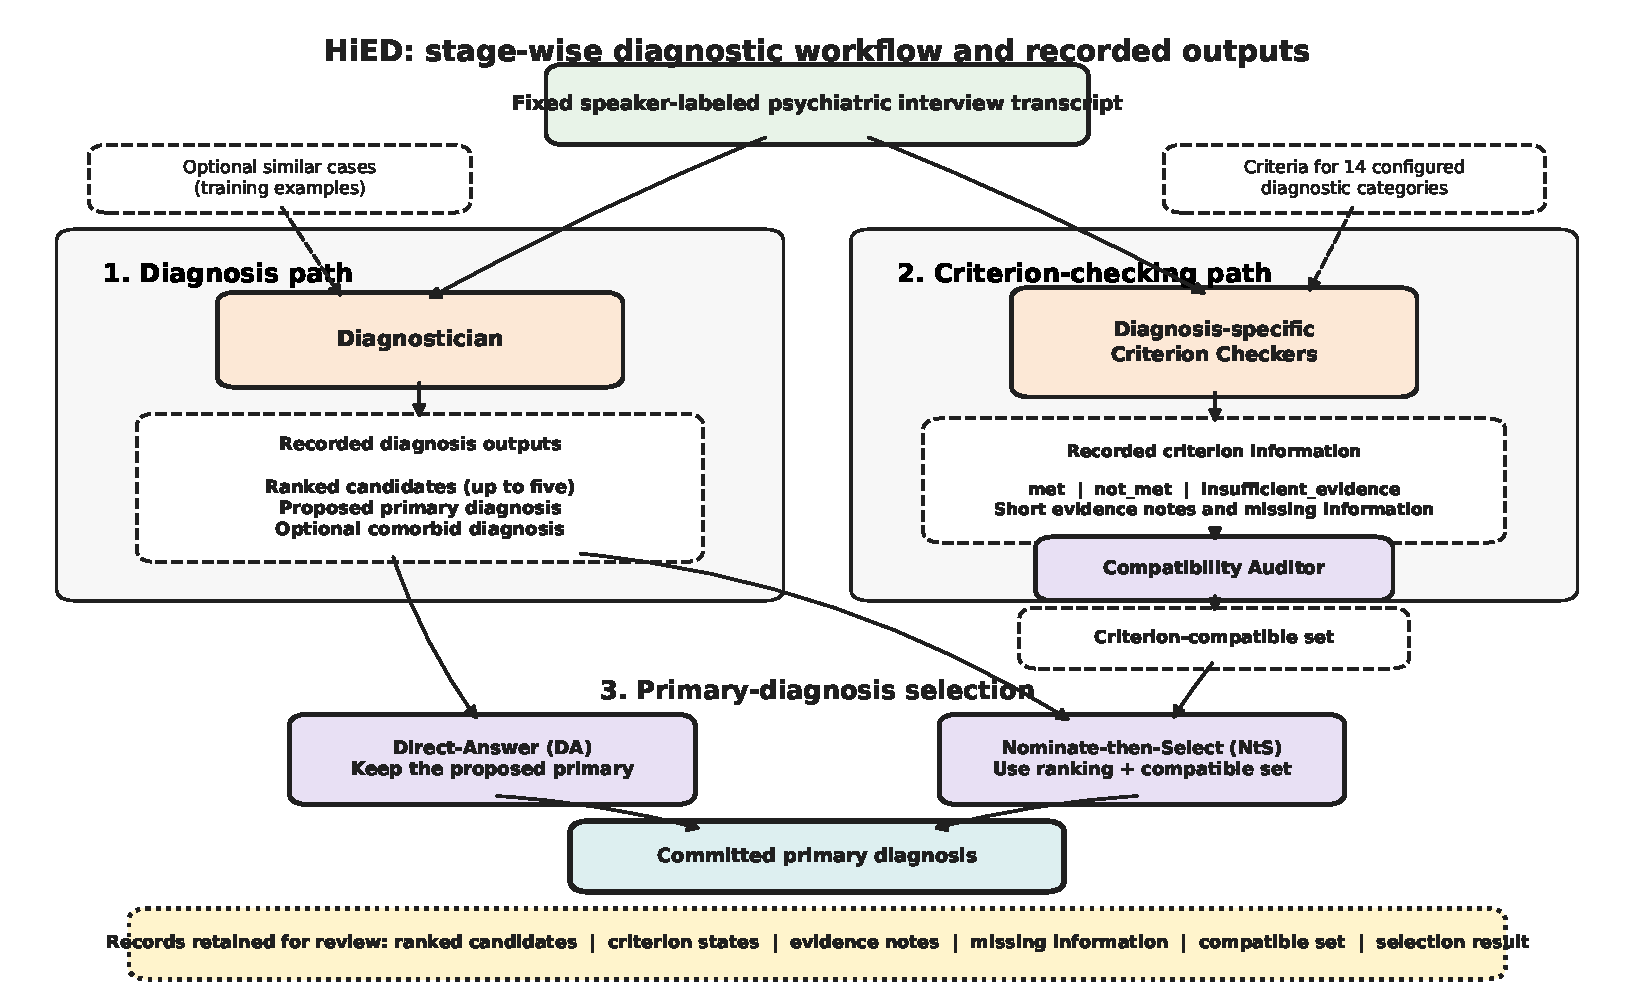
\includegraphics[width=1.0\textwidth]{fig_hied_two_path_architecture.pdf}
\caption{HiED two-path architecture and recorded diagnostic outputs. The fixed transcript is processed by a diagnosis path and a criterion-checking path. Similar cases, when used, are provided only to the diagnosis path. The diagnosis path records ranked candidates and a proposed primary diagnosis. The criterion-checking path records criterion states, evidence notes, missing information, and a criterion-compatible set. Direct-Answer keeps the proposed primary, whereas Nominate-then-Select uses the ranking and compatible set to reselect the committed primary. All intermediate records remain available for review.}
\label{fig:hied-two-path-architecture}
\label{fig:single-vs-hied-architecture}
\label{fig:pipeline-thesis-rewrite}
\end{figure}
\FloatBarrier

\section{Diagnosis Path: Candidate Formation and Primary Proposal}
\label{sec:retrieval}
\label{sec:diagnosis-path}

The diagnosis path forms a differential diagnosis from the fixed transcript. Its main outputs are a ranked candidate list, a proposed primary diagnosis, and an optional comorbid diagnosis.

\subsection{Optional Similar-Case Retrieval}

When retrieval is enabled, similar labeled cases are provided only to the diagnosis path. They may guide candidate formation and the proposed primary diagnosis, but they do not change the current transcript or the input to the Criterion Checkers. The retrieval policies and their evaluation are described in Chapter~\ref{ch:experimental}.

\subsection{Diagnostician Outputs}
\label{sec:diagnostician-outputs}

The Diagnostician receives the speaker-labeled transcript, the configured diagnostic scope, and any retrieved examples. It records:

\begin{enumerate}
    \item a ranked list of up to five candidate diagnoses;
    \item one proposed primary diagnosis selected from the leading candidates; and
    \item at most one optional comorbid diagnosis.
\end{enumerate}

The ranked list keeps possible alternatives visible even when they are not selected as primary. The proposed primary diagnosis is the Diagnostician's direct first choice. The optional comorbid diagnosis has a different role: it proposes that another disorder may be present at the same time. A diagnosis in the ranked list is therefore not automatically a comorbidity.

These three outputs come from the same Diagnostician and should not be treated as independent model opinions. They are kept separately because candidate availability, primary preference, and comorbidity are different diagnostic roles.

\section{Criterion-Checking Path: Criterion States and Compatibility}
\label{sec:criterion-checking-path}

The criterion-checking path examines the transcript at the diagnostic criterion level. It asks whether each configured diagnosis is compatible with the evidence in the fixed transcript. It does not rank the compatible diagnoses or decide which one should be primary.

\subsection{Diagnosis-Specific Criterion Checkers}
\label{sec:criterion-checkers}

Each of the fourteen configured diagnostic categories has its own Criterion Checker. Every checker receives the same speaker-labeled transcript together with the study-specific criteria for one diagnosis. The checkers do not receive the retrieved similar-case examples, and they do not use the Diagnostician's ranked candidate list.

All fourteen categories are checked for every case. A diagnosis may therefore enter the criterion-compatible set even when it was not ranked among the leading candidates.

For each criterion, the checker records one of three states. Table~\ref{tab:criterion-state-definitions} gives their meanings.

\begin{table}[htbp]
\centering
\caption{Criterion states recorded by the Criterion Checkers.}
\label{tab:criterion-state-definitions}
\small
\begin{tabularx}{\textwidth}{|>{\raggedright\arraybackslash}p{3.6cm}|>{\raggedright\arraybackslash}X|}
\hline
\textbf{Criterion state} & \textbf{Meaning in this study}\\
\hline
\texttt{met} & The transcript contains information that supports the criterion.\\
\hline
\texttt{not\_met} & The transcript contains information showing that the criterion is not met.\\
\hline
\texttt{insufficient\_\allowbreak{}evidence} & The transcript does not contain enough information to decide whether the criterion is met.\\
\hline
\end{tabularx}
\end{table}

An \texttt{insufficient\_\allowbreak{}evidence} state is not treated as negative evidence. It means that the current transcript does not provide enough information for either a \texttt{met} or a \texttt{not\_met} judgment. When relevant information is found, the checker also records a short evidence note for later review.

\subsection{Compatibility Auditor}
\label{sec:compatibility-auditor}

After the Criterion Checkers finish, a deterministic Compatibility Auditor applies the study-specific rule for each diagnosis. A rule may require particular core criteria, a minimum number of supported criteria, a required duration, or a combination of these conditions.

The auditor uses only the recorded criterion states. It does not reread the transcript or create new evidence. Diagnoses that pass their configured rules are placed in the criterion-compatible set. The complete rules are reported in Appendix~\ref{app:configured-profile}.

\subsection{Meaning of Criterion Compatibility}
\label{sec:criterion-compatibility-boundary}

A compatible diagnosis has passed the study-specific rule using the recorded criterion states. This does not show that it is clinically correct, mutually exclusive with other diagnoses, or the preferred primary diagnosis. Compatibility records whether one diagnosis fits its own rule; primary selection compares several possible diagnoses.

\section{Primary-Diagnosis Selection}
\label{sec:primary-selection}

The diagnosis and criterion-checking paths provide different views of the same transcript. The primary-selection step records which diagnosis is finally committed as the system output.

\subsection{Direct-Answer Policy}
\label{sec:direct-answer-policy}

Direct-Answer (DA) keeps the Diagnostician's proposed primary diagnosis as the committed primary diagnosis. The criterion records and criterion-compatible set remain available for review but do not replace that choice. DA may also retain one optional comorbid diagnosis.

\subsection{Nominate-then-Select Policy}
\label{sec:nominate-then-select-policy}

Nominate-then-Select (NtS) reselects the committed primary diagnosis using the ranked candidates and the criterion-compatible set. It returns one committed primary diagnosis and does not retain DA's optional comorbid output. The complete fallback order and tie-handling rules are reported in the experimental protocol and appendix.

\subsection{Shared Upstream Records and Comparison Boundary}
\label{sec:da-nts-relationship}
\label{sec:primary-selection-boundary}

DA and NtS reuse the same ranked candidates, proposed primary diagnosis, criterion states, and criterion-compatible set. Their difference is how these records are used to commit one primary diagnosis. Their committed Top-1 results can therefore be compared directly. Set-based measures also reflect their different output sizes because DA may retain a comorbid diagnosis whereas NtS returns one diagnosis.

The committed primary is the system's benchmark output. A mismatch with a gold label may reflect an unsuitable system choice, missing transcript information, or ambiguity in the dataset label. This thesis therefore reports benchmark agreement and disagreement rather than treating every mismatch as a confirmed clinical error.

\section{Single LLM Baseline and Comparison Contract}
\label{sec:compared-architectures}

\subsection{Single LLM Baseline}
\label{sec:single-architecture}

The Single LLM receives the same fixed transcript and optional similar-case examples. It returns a primary diagnosis and may emit additional diagnostic labels. These additional labels are not produced as the same ranked differential used by HiED, and the Single LLM does not produce a diagnosis-specific criterion record.

The Single LLM is therefore used as a direct diagnostic baseline. Its final diagnostic outputs can be compared with HiED, but its emitted labels cannot be treated as the same stage-wise records.

\subsection{Recorded Output Comparison}
\label{sec:recorded-output-differences}

Table~\ref{tab:single-hied-output-comparison} summarizes the outputs available from the two study architectures.

\begin{table}[htbp]
\centering
\caption{Recorded outputs available from the Single LLM and HiED study architectures.}
\label{tab:single-hied-output-comparison}
\footnotesize
\begin{tabularx}{\textwidth}{|>{\raggedright\arraybackslash}p{4.2cm}|>{\centering\arraybackslash}p{3.0cm}|>{\centering\arraybackslash}X|}
\hline
\textbf{Recorded output} & \textbf{Single LLM} & \textbf{HiED}\\
\hline
Committed primary diagnosis & Yes & Yes\\
\hline
Optional additional diagnosis & Possible under the Single format & Optional comorbid diagnosis\\
\hline
Genuine ranked differential diagnosis & No & Yes\\
\hline
Criterion state for each configured diagnosis & No & Yes\\
\hline
Evidence notes and missing-information record & No & Yes\\
\hline
Criterion-compatible diagnosis set & No & Yes\\
\hline
Separately observable diagnostic stages & Final emitted output only & Candidate generation, criterion checking, and primary selection\\
\hline
\end{tabularx}
\end{table}

The comparison concerns complete study architectures, not the isolated effect of agent count. The systems differ in workflow, model calls, intermediate outputs, and output contract.

\section{Complete Worked Example}
\label{sec:running-example}
\label{sec:worked-example}

\subsection{Example Purpose and Overview}

This section follows one complete constructed psychiatric interview through the Single LLM and HiED output contracts. The transcript is written for this thesis. It is not a patient record, a case copied from LingxiDiag, or an exported model trace. The example is used only to explain the data flow and output roles.

Figure~\ref{fig:worked-example-flow} provides an overview before the complete transcript and output tables. Only selected categories are shown in the figure, although the full HiED configuration checks all fourteen categories.

\begin{figure}[htbp]
\centering
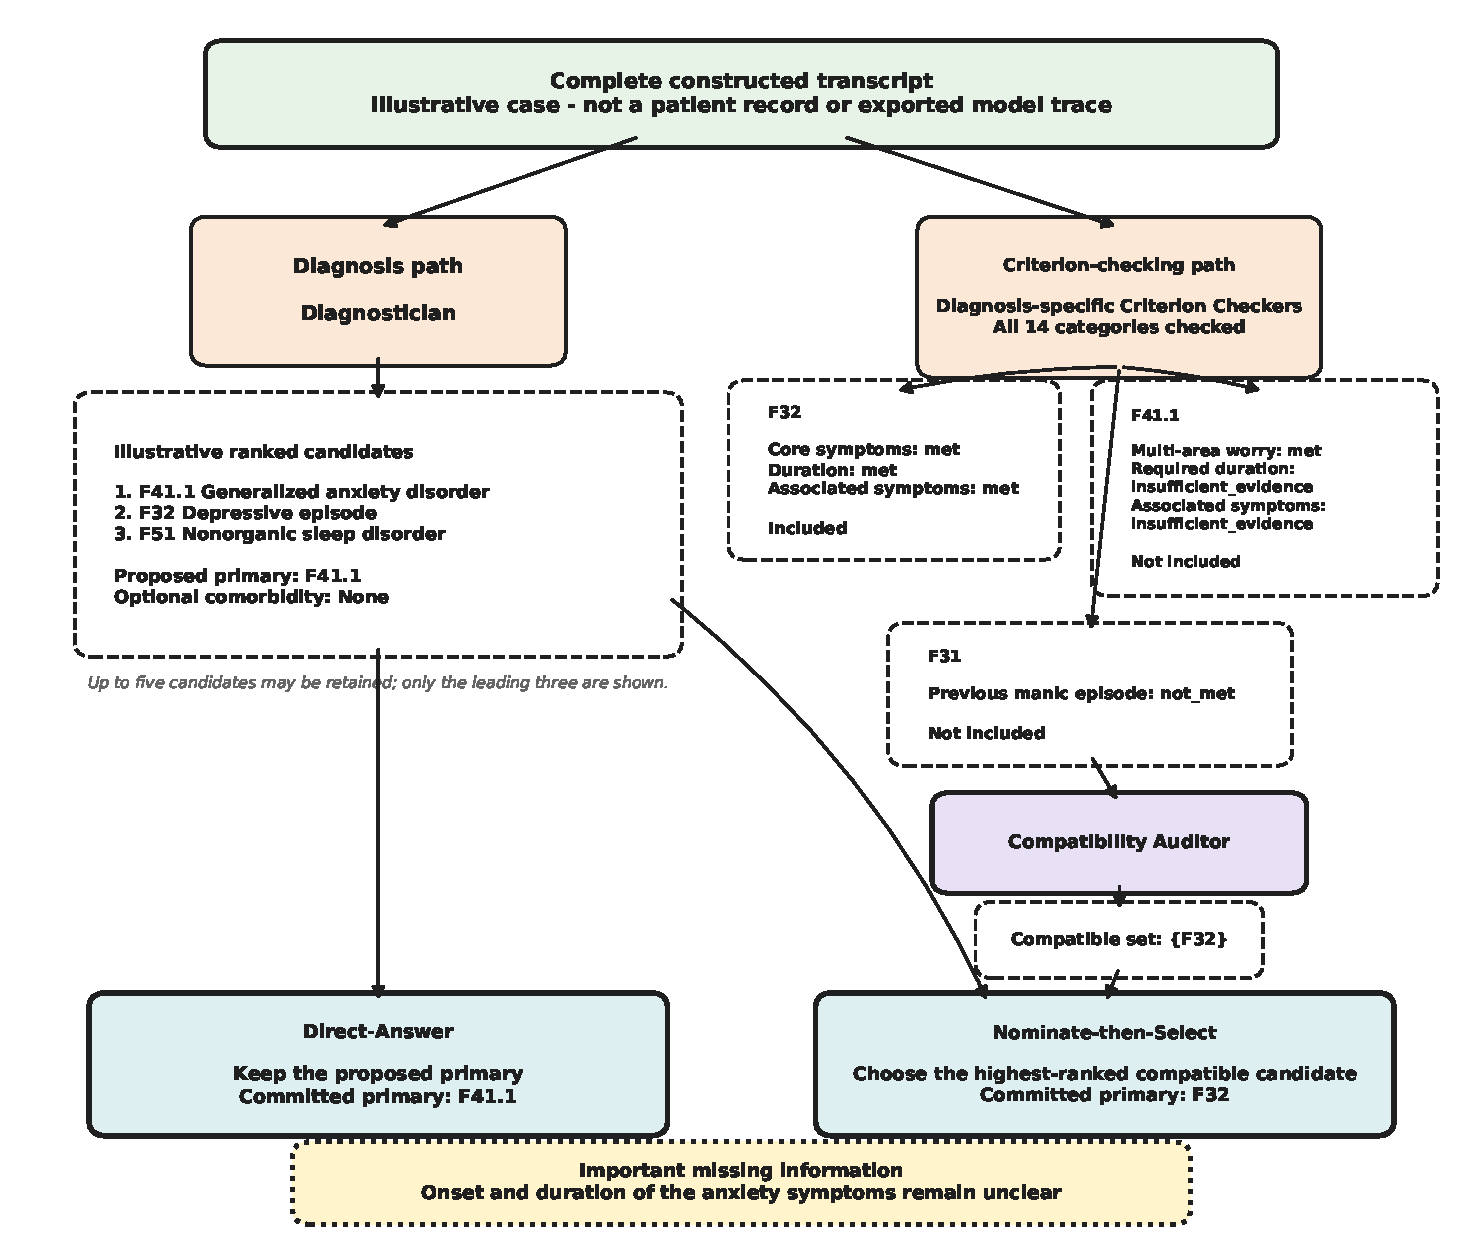
\includegraphics[width=1.0\textwidth]{fig_worked_example_flow.pdf}
\caption{Illustrative HiED data flow for the complete constructed psychiatric interview. The diagnosis path ranks F41.1 above F32 and proposes F41.1 as primary. In the selected criterion records, F32 passes the configured compatibility rule, whereas the duration and associated symptoms required for F41.1 remain unclear. Direct-Answer keeps the proposed F41.1 primary diagnosis, while Nominate-then-Select commits F32 using the same upstream outputs. The example explains the output contract and does not represent a patient record, benchmark result, or clinically adjudicated diagnosis.}
\label{fig:worked-example-flow}
\end{figure}
\FloatBarrier

\subsection{Complete Constructed Transcript}

Table~\ref{tab:worked-example-transcript} presents the complete speaker-labeled transcript used in this worked example.

{\small
\begin{longtable}{|>{\raggedright\arraybackslash}p{1.6cm}|>{\raggedright\arraybackslash}p{6.1cm}|>{\raggedright\arraybackslash}p{6.1cm}|}
\caption{Complete constructed psychiatric interview used in the worked example.}
\label{tab:worked-example-transcript}\\
\hline
\textbf{Speaker} & \textbf{Original Chinese utterance} & \textbf{English translation}\\
\hline
\endfirsthead
\multicolumn{3}{c}{\tablename\ \thetable\ -- continued from the previous page}\\
\hline
\textbf{Speaker} & \textbf{Original Chinese utterance} & \textbf{English translation}\\
\hline
\endhead
Clinician & 最近最困擾你的事情是什麼？ & What has been troubling you most recently?\\
\hline
Patient & 這兩個星期幾乎每天心情都很低落，原本喜歡做的事情也都不想做。 & For the past two weeks, I have felt low almost every day and no longer want to do things that I previously enjoyed.\\
\hline
Clinician & 睡眠、食慾、精神和專注力有受到影響嗎？ & Have your sleep, appetite, energy, or concentration been affected?\\
\hline
Patient & 我常常很早就醒來，食慾也變差，整天沒有力氣，上班很難專心，做事情比以前慢很多。 & I often wake up very early, have less appetite, feel tired throughout the day, and have difficulty concentrating at work. I also work much more slowly than before.\\
\hline
Clinician & 最近會不會常覺得自己很沒用，或一直責怪自己？ & Have you often felt useless or blamed yourself recently?\\
\hline
Patient & 會，我覺得自己工作做不好，也沒有把家裡照顧好，常常覺得都是我的問題。 & Yes. I feel that I am doing poorly at work and not taking good care of my family. I often feel that everything is my fault.\\
\hline
Clinician & 你也提到會擔心。通常擔心哪些事情？持續多久了？ & You also mentioned feeling worried. What do you usually worry about, and how long has this continued?\\
\hline
Patient & 工作和家裡的事情都會擔心，腦子很難停下來，但我不確定是從什麼時候開始。好像心情變差後變得比較明顯。 & I worry about both work and family and find it difficult to stop thinking, but I am unsure when it began. It seems to have become more noticeable after my mood worsened.\\
\hline
Clinician & 擔心的時候，有沒有明顯坐立不安、肌肉緊繃、心悸或冒汗？ & When you feel worried, do you have clear restlessness, muscle tension, palpitations, or sweating?\\
\hline
Patient & 有時候肩膀很緊，心跳也會快一點，但不是每次都有，我自己也不太確定。 & Sometimes my shoulders feel tense and my heartbeat becomes faster, but this does not happen every time, and I am not very sure about it.\\
\hline
Clinician & 有沒有突然出現很強烈的害怕，幾分鐘內心跳很快、喘不過氣，覺得自己快要失控？ & Have you had sudden episodes of intense fear, with a rapid heartbeat, shortness of breath, or a feeling that you were losing control within a few minutes?\\
\hline
Patient & 沒有，沒有那種突然發作的情況。 & No. I have not had that kind of sudden episode.\\
\hline
Clinician & 以前有沒有一段時間特別亢奮、話很多、活動明顯增加，睡得很少也不覺得累？ & Have you ever had a period of unusually elevated mood, increased talking or activity, and very little sleep without feeling tired?\\
\hline
Patient & 沒有，我以前沒有這種情況。 & No. I have never experienced that.\\
\hline
Clinician & 最近有沒有聽到別人聽不到的聲音，或覺得有人要害你？ & Have you recently heard voices that other people could not hear, or felt that someone wanted to harm you?\\
\hline
Patient & 沒有。 & No.\\
\hline
Clinician & 最近有沒有大量喝酒、使用其他物質、開始新的藥物，或出現其他明顯的身體疾病？ & Have you recently used a large amount of alcohol, used other substances, started a new medication, or developed a clear medical problem?\\
\hline
Patient & 偶爾會喝一點酒，沒有用其他東西，也沒有開始新的藥。目前沒有知道的重大身體疾病。 & I occasionally drink a small amount of alcohol. I do not use other substances and have not started a new medication. I do not know of any major medical condition.\\
\hline
Clinician & 最近有沒有覺得活著沒有意義，或想過傷害自己？ & Have you recently felt that life was meaningless or thought about harming yourself?\\
\hline
Patient & 有時候會覺得很沒希望，但沒有想過傷害自己，也沒有計畫。 & I sometimes feel hopeless, but I have not thought about harming myself and have no plan.\\
\hline
Clinician & 以前有過類似的情況嗎？有沒有接受過精神科治療？ & Have you experienced a similar period before, or received psychiatric treatment?\\
\hline
Patient & 以前壓力大時會睡不好，但沒有像這次這麼嚴重，也沒有看過精神科。 & I have had poor sleep during stressful periods, but it was never this severe, and I have not received psychiatric treatment.\\
\hline
\end{longtable}
}

\subsection{Illustrative Single LLM Output}

Under the Single LLM output contract, an illustrative output for this transcript is shown in Table~\ref{tab:worked-example-single}.

\begin{table}[htbp]
\centering
\caption{Illustrative Single LLM output for the constructed transcript.}
\label{tab:worked-example-single}
\small
\begin{tabularx}{0.82\textwidth}{|>{\raggedright\arraybackslash}p{4.0cm}|>{\raggedright\arraybackslash}X|}
\hline
\textbf{Output field} & \textbf{Illustrative output}\\
\hline
Primary diagnosis & F41.1 Generalized anxiety disorder\\
\hline
Optional additional diagnosis & F32 Depressive episode\\
\hline
Diagnosis-specific criterion states & Not produced\\
\hline
Standardized ranked differential & Not produced under this contract\\
\hline
\end{tabularx}
\end{table}

The additional F32 label is an emitted diagnostic label, not a standardized rank-two candidate under the HiED ranking contract. Therefore, the Single output should not be interpreted as the same ranked differential produced by HiED.

\subsection{Diagnosis-Path Outputs}

The diagnosis path keeps the candidate ranking and proposed primary diagnosis as separate outputs.

\begin{table}[htbp]
\centering
\caption{Illustrative diagnosis-path output for the constructed transcript.}
\label{tab:worked-example-diagnosis-path}
\small
\begin{tabularx}{0.86\textwidth}{|>{\raggedright\arraybackslash}p{4.1cm}|>{\raggedright\arraybackslash}X|}
\hline
\textbf{Output role} & \textbf{Illustrative output}\\
\hline
Rank 1 & F41.1 Generalized anxiety disorder\\
\hline
Rank 2 & F32 Depressive episode\\
\hline
Rank 3 & F51 Nonorganic sleep disorder\\
\hline
Proposed primary diagnosis & F41.1 Generalized anxiety disorder\\
\hline
Optional comorbid diagnosis & None\\
\hline
\end{tabularx}
\end{table}

The ranking keeps F32 visible even though F41.1 is proposed as primary. This separation allows candidate availability and primary selection to be examined as different output views.

\subsection{Criterion States and Missing Information}

Table~\ref{tab:worked-example-criteria} presents selected criterion states for three diagnoses. The states are illustrative applications of the study rules.

\begin{table}[htbp]
\centering
\caption{Selected illustrative criterion states for the constructed transcript.}
\label{tab:worked-example-criteria}
\footnotesize
\begin{tabularx}{\textwidth}{|>{\raggedright\arraybackslash}p{2.5cm}|>{\raggedright\arraybackslash}p{3.7cm}|>{\centering\arraybackslash}p{2.9cm}|>{\raggedright\arraybackslash}X|}
\hline
\textbf{Diagnosis} & \textbf{Criterion or evidence need} & \textbf{State} & \textbf{Information from the transcript}\\
\hline
F32 & Depressed mood and loss of interest & \texttt{met} & Both are reported almost every day.\\
\hline
F32 & Duration of at least two weeks & \texttt{met} & The patient reports a two-week period.\\
\hline
F32 & Associated symptoms and functional effect & \texttt{met} & Early waking, reduced appetite, low energy, poor concentration, self-blame, and reduced work function are reported.\\
\hline
F41.1 & Worry across more than one area & \texttt{met} & The patient reports worry about work and family.\\
\hline
F41.1 & Required duration & \shortstack{\scriptsize\texttt{insufficient\_}\\\scriptsize\texttt{evidence}} & The patient cannot state when the worry began.\\
\hline
F41.1 & Associated anxiety symptoms & \shortstack{\scriptsize\texttt{insufficient\_}\\\scriptsize\texttt{evidence}} & Some tension and increased heartbeat are reported, but their pattern and frequency remain unclear.\\
\hline
F31 & Previous manic episode & \texttt{not\_met} & The patient denies past elevated mood, increased activity, and reduced need for sleep.\\
\hline
\end{tabularx}
\end{table}

Under the illustrative criterion states, F32 passes the configured compatibility rule. F41.1 does not enter the criterion-compatible set because the required duration remains unclear. F31 does not pass because no previous manic episode is supported.

\subsection{DA and NtS Selection Results}

\begin{table}[htbp]
\centering
\caption{Illustrative compatibility and finalization outputs.}
\label{tab:running-example}
\label{tab:worked-example-finalization}
\small
\begin{tabularx}{0.9\textwidth}{|>{\raggedright\arraybackslash}p{4.2cm}|>{\raggedright\arraybackslash}X|}
\hline
\textbf{Output} & \textbf{Illustrative result}\\
\hline
Criterion-compatible set & \{F32\}\\
\hline
Diagnostician proposed primary & F41.1\\
\hline
DA committed primary & F41.1\\
\hline
NtS committed primary & F32\\
\hline
Remaining important uncertainty & The onset and duration of the anxiety symptoms remain unclear.\\
\hline
\end{tabularx}
\end{table}



DA keeps the Diagnostician's proposed primary diagnosis. NtS selects the highest-ranked diagnosis that also passes the compatibility rule. The two policies therefore produce different committed primary diagnoses while using the same transcript, ranking, and criterion states.

\subsection{What the Example Demonstrates}

This worked example demonstrates four features of the study architecture.

First, a diagnosis may remain visible in the ranked differential even when it is not proposed as primary. Second, criterion checking may support one diagnosis while leaving another diagnosis unresolved because important information is missing. Third, criterion compatibility and primary selection are different decisions. Fourth, DA and NtS may produce different committed diagnoses from the same upstream outputs.

The example does not establish that F32 is the clinically correct diagnosis or that NtS is a better policy. It contains no benchmark gold label and is not part of the quantitative evaluation. In the aggregate experiments, NtS does not consistently improve committed-primary agreement. The example is used only to make the architecture and output roles concrete.

\section{Chapter Summary}

HiED processes one fixed transcript within a fourteen-category diagnostic space. It separately records ranked candidates, criterion states, evidence notes, missing information, criterion compatibility, and the committed primary diagnosis.

The diagnosis path forms and ranks possible diagnoses and proposes a primary diagnosis. The criterion-checking path evaluates all configured categories and records which criteria are supported, contradicted, or unclear. A deterministic Compatibility Auditor then forms the criterion-compatible set.

DA and NtS use the same upstream records in different ways during primary selection. DA keeps the proposed primary diagnosis, whereas NtS uses the ranking and criterion-compatible set to make a new selection. The Single LLM provides a direct diagnostic baseline but does not provide the same stage-wise output contract.

The worked example showed how the same transcript can produce a ranked differential, criterion-level records, missing-information states, and different DA and NtS commitments. These records form the basis of the stage-wise evaluation defined in the following chapters.

\chapter{Datasets, Label Projection, and Evaluation Protocol}
\label{ch:data}

\section{Configured Output Space and Gold-Label Projection}
\label{sec:gold-label-conventions}

Throughout this thesis, the dataset-provided diagnoses used for scoring are referred to as \emph{benchmark gold labels}. The term \emph{gold} denotes the official benchmark reference and does not imply a uniquely correct clinical diagnosis.

The main system uses fourteen configured ICD-10 diagnostic categories, listed in Table~\ref{tab:configured-profile-summary}. For evaluation, subtype-level categories are projected to eleven broader parent labels. Let $G_{\mathrm{raw}}(x)$ be the raw benchmark gold codes for case $x$, and let $\pi$ map subtype-level codes to their scoring parents, mapping F41.0, F41.1, and F41.2 to F41 and F43.1 and F43.2 to F43. Codes already defined at the scoring-parent level are left unchanged. Let $\mathcal{C}$ be the set of eleven configured scoring parents. The in-scope gold-label set is
\[
G_{\mathrm{in}}(x)=\{\pi(c):c\in G_{\mathrm{raw}}(x),\ \pi(c)\in\mathcal{C}\}.
\]
The scored gold-label set is then
\[
G(x)=
\begin{cases}
G_{\mathrm{in}}(x), & G_{\mathrm{in}}(x)\neq\varnothing,\\
\{\mathrm{Others}\}, & G_{\mathrm{in}}(x)=\varnothing.
\end{cases}
\]
Thus, when a case contains both an out-of-scope code and F41.1, its scored gold-label set is $\{\mathrm{F41}\}$ rather than $\{\mathrm{Others},\mathrm{F41}\}$. A case is in scope when $G_{\mathrm{in}}(x)$ is nonempty and out of scope otherwise. Because the main system has neither an \emph{Others} output nor a trained unknown detector, it cannot correctly represent an out-of-scope case.

For case $x$, $G(x)$ is the deduplicated gold-label set after parent-level projection; we refer to the individual labels in $G(x)$ as \emph{benchmark gold parents}. LingxiDiag cases may contain more than one gold parent label, and neither dataset provides a psychiatrist-reviewed unique clinical primary diagnosis. The first-listed gold parent is used only for explicitly single-label descriptive analyses such as the confusion matrix.

\section{Datasets, Case Construction, and Split Roles}

The study uses two synthetic Chinese psychiatric dialogue datasets. LingxiDiag-16K, the dataset underlying LingxiDiagBench, is used for system development and internal held-out evaluation, whereas MDD-5k is used for external cross-dataset evaluation.

\subsection{LingxiDiag-16K}

LingxiDiag-16K is the synthetic Chinese psychiatric dialogue dataset underlying LingxiDiagBench and was generated for static diagnostic classification and interactive consultation tasks~\citep{xu2026lingxidiagbench}. It provides a fixed diagnostic label space and sufficient cases for training, configuration selection, and internal held-out evaluation. The published LingxiDiagBench results also show that fine-grained disorder-level diagnosis is substantially more difficult than broad depression--anxiety classification.

The accessible release used in this study contained 14,000 training-source cases and 1,000 public-validation cases. The official test file was not available in the accessible release used when the experiments were designed.

The 1,000-case internal held-out set was sampled from the 14,000-case training source using the first-listed projected parent label to approximately match the public-validation class distribution. A fixed random seed was used for reproducibility. The remaining 13,000 cases define the required training source for a leakage-controlled conventional baseline and were used to build the retained retrieval index. The first-listed label served only as a stratification variable and was not treated as a clinically validated primary diagnosis. Case-ID checks confirmed that held-out cases were excluded from the retained Route B system runs, the retrieval index, and all configuration-selection procedures. No additional semantic near-duplicate screening was performed. The preserved legacy S8 TF--IDF artifact predates this split convention: it was trained on the full 14,000-case source and evaluated on the disjoint public-validation split. It is therefore reported only as validation-split evidence and is not used as a Route B baseline.

\begin{table}[htbp]
\centering
\caption{LingxiDiag-16K data splits and their roles in this thesis.}
\label{tab:data-roles-rewrite}
\small
\begin{tabularx}{\textwidth}{|>{\raggedright\arraybackslash}p{3.7cm}|r|>{\raggedright\arraybackslash}X|}
\hline
Split & $N$ & Role\\
\hline
Route B training source & 13,000 & Required source for leakage-controlled conventional baselines and used to build the retrieval index; no retained TF--IDF Route B run is reported\\
\hline
Public validation & 1,000 & Supports prompt, rule, sensitivity, and retrieval-configuration selection; reported only as descriptive development-set context\\
\hline
Internal held-out set & 1,000 & Provides the main internal performance estimate after configuration selection\\
\hline
\end{tabularx}
\end{table}

All methods in the main Route B table are reported on the same fixed 1,000-case held-out set. The preserved TF--IDF analysis is explicitly separated because it evaluates the public-validation cases. Because the public-validation split was also used during system development, its results are descriptive development evidence rather than an independent test estimate.

\subsection{MDD-5k}

MDD-5k is a synthetic Chinese psychiatric dialogue dataset generated from anonymized psychiatric case information through a neuro-symbolic multi-agent process~\citep{yin2024mdd5k}. Some patient files contain multiple dialogue rounds. The study adapter concatenates these rounds in their recorded order while preserving doctor and patient turns, and each patient file is treated as one evaluation case.

The evaluated release contains 925 patient-level cases. Under HiED's main configured output space defined in Section~\ref{sec:gold-label-conventions}, a case is defined as \emph{in scope} when at least one projected benchmark gold diagnosis can be emitted by the system and as \emph{out of scope} when none of its projected gold diagnoses is represented in that output space. Among the 925 external cases, 878 are in scope and the remaining 47 are out of scope. Because MDD-5k transcripts are generally longer than those in LingxiDiag-16K, the external runs use the same deterministic, turn-preserving prompt-budget procedure as the internal runs; the implementation rule is reported in Appendix~\ref{app:supporting}. MDD-5k is used as an external synthetic benchmark and does not constitute validation on real patient transcripts.

\subsection{Evaluation-Set Label Distributions}

Table~\ref{tab:class-distribution} provides a descriptive view of the label composition of the internal and external evaluation populations. The distribution is reported to clarify class imbalance, the dominance of the F32 and F41 categories, and the different role of out-of-scope cases across the two corpora.

\begin{table}[htbp]
\centering
\caption{Distribution of first-listed projected gold labels across the internal and external synthetic evaluation sets.}
\label{tab:class-distribution}
\small
\begin{adjustbox}{max width=\textwidth}
\begin{tabular}{|l|l|r|r|r|}
\hline
Scoring label & Label description &
\shortstack{\rule{0pt}{2.4ex}Internal test\\($N=1000$)} &
\shortstack{\rule{0pt}{2.4ex}MDD-5k in-scope\\($N=878$)} &
\shortstack{\rule{0pt}{2.4ex}MDD-5k out-of-scope\\($N=47$)}\\
\hline
F20 & Schizophrenia & 5 & 3 & 0\\
\hline
F31 & Bipolar affective disorder & 9 & 11 & 0\\
\hline
F32 & Depressive episode & 365 & 410 & 0\\
\hline
F39 & Unspecified mood disorder & 60 & 64 & 0\\
\hline
F41 & Anxiety disorders & 358 & 313 & 0\\
\hline
F42 & Obsessive-compulsive disorder & 25 & 13 & 0\\
\hline
F43 & Stress-related disorders & 11 & 7 & 0\\
\hline
F45 & Somatoform disorders & 8 & 7 & 0\\
\hline
F51 & Nonorganic sleep disorders & 36 & 18 & 0\\
\hline
F98 & Other behavioral and emotional disorders & 30 & 24 & 0\\
\hline
Z71 & Counseling without a specific disorder & 8 & 8 & 0\\
\hline
Others & Out-of-scope gold diagnosis & 85 & 0 & 47\\
\hline
 & Total & 1000 & 878 & 47\\
\hline
\end{tabular}
\end{adjustbox}
\end{table}

\noindent\textit{Note:} Cases may contain more than one projected gold label. For this descriptive distribution, each case is assigned to its first-listed projected gold label so that each column sums to the corresponding number of cases. The table therefore does not report multilabel prevalence. \emph{Others} is an evaluation category assigned when none of a case's dataset gold diagnoses is represented in the configured output space; it is not a diagnosis that HiED can emit.

F32 and F41 make up most cases in both the internal held-out set and the in-scope \mbox{MDD-5k} subset, while several other categories contain only a small number of cases. Consequently, support-weighted measures such as Weighted-F1 are driven mainly by performance on F32 and F41 and may underrepresent performance on less frequent categories.

\section{Prediction Views and Metrics}
\label{sec:prediction-metrics}

The evaluator keeps five recorded output views separate:

\begin{enumerate}[label=(\arabic*)]
\item The \emph{primary view}, $p_1(x)$, is the committed primary diagnosis.
\item The \emph{ranked view}, $R_3(x)$, contains the first three distinct parent labels in a method's genuine ranked output. TF--IDF with logistic regression obtains this view from ranked class scores. HiED obtains it from the recorded Diagnostician ranking, before DA or NtS finalization.
\item The \emph{emitted-label sequence}, $E_3(x)$, contains the first three distinct parent labels available in the final emitted output, with the committed primary diagnosis placed first. This view is used only when aggregate benchmark reporting requires a three-label hit rate but the method does not produce a genuine ranking.
\item The \emph{compatibility view}, $L(x)$, is the set of scoring parent labels classified as criterion-compatible by the Compatibility Auditor under the configured operational rules.
\item The \emph{multilabel view}, $M(x)$, is the complete set of emitted parent labels used for Exact Match and F1. For DA, it contains the committed primary diagnosis and any emitted comorbid parent label. For a single-label method, it contains one label.
\end{enumerate}

Within a method, Exact Match, Macro-F1, and Weighted-F1 are computed from the identical multilabel set $M(x)$. No metric-specific threshold or Top-1 substitution is used: a score threshold matters only insofar as it defines $M(x)$ before all three set-based measures are calculated.

Single does not produce a standardized ranked differential diagnosis, so it has no genuine $R_3(x)$ view. For continuity with the aggregate LingxiDiagBench reporting convention, this thesis separately reports an \emph{emitted-label hit@3} from $E_3(x)$ for Single. The sequence may contain an optional additional diagnosis that was emitted as a comorbidity rather than ranked as a differential alternative. It is therefore not interpreted as candidate coverage and is not used to define $D_3$. The Majority baseline emits one label, so its emitted-label hit@3 is numerically identical to its Top-1 Accuracy.

Because a case may contain more than one gold label, each hit measure counts a case as correct when at least one projected benchmark gold label appears in the evaluated view. Exact Match, also called subset accuracy, instead requires the complete predicted label set to equal the complete gold-label set. These are benchmark-agreement measures, not independent measures of the patient's true clinical diagnosis.

For example, suppose that the projected gold-label set contains F41, while a genuine ranking places F32 first and F41.1 second. Because F41.1 is projected to its scoring parent F41, the case is incorrect under committed Top-1 evaluation but correct under ranked Top-3 evaluation.

DA may emit a committed primary diagnosis and one optional comorbid diagnosis, whereas NtS emits one committed primary diagnosis. Their Top-1 comparison therefore evaluates the committed primary directly, but differences in Exact Match, Macro-F1, or Weighted-F1 also reflect output cardinality and cannot be interpreted as isolated effects of primary re-selection.

Table~\ref{tab:metric-contract} summarizes which recorded output view is evaluated by each measure. The subsequent equations give the case-level definitions used by the scoring implementation.

\begin{table}[H]
\centering
\caption{Definitions of the main evaluation measures by output view.}
\label{tab:metric-contract}
\small
\begin{tabularx}{\textwidth}{|>{\raggedright\arraybackslash}p{3.2cm}|>{\raggedright\arraybackslash}p{3.8cm}|>{\raggedright\arraybackslash}X|}
\hline
Measure & Evaluated output & Definition\\
\hline
Top-1 Accuracy & Committed primary, $p_1(x)$ & $p_1(x)\in G(x)$\\
\hline
Ranked Top-3 Accuracy & Genuine ranked candidates, $R_3(x)$ & $R_3(x)\cap G(x)\neq\varnothing$\\
\hline
Emitted-label hit@3 & Emitted-label sequence, $E_3(x)$ & $E_3(x)\cap G(x)\neq\varnothing$\\
\hline
Gold-label inclusion & Criterion-compatible set, $L(x)$ & $L(x)\cap G(x)\neq\varnothing$\\
\hline
Exact Match & Complete emitted set, $M(x)$ & $M(x)=G(x)$\\
\hline
Macro-F1 & Complete emitted set, $M(x)$ & Unweighted mean of the fixed-class one-vs-rest F1 scores\\
\hline
Weighted-F1 & Complete emitted set, $M(x)$ & The same label-level F1 scores weighted by gold-label support\\
\hline
\end{tabularx}
\end{table}

Top-1 and any reported three-label hit measure are computed over all 1,000 internal test cases. Ranked Top-3 is reported only for a method with a genuine ranked view. Gold-label inclusion in the criterion-compatible set is computed over the 915 cases with at least one non-\emph{Others} gold parent covered by a corresponding Criterion Checker.

\[
\mathrm{Top\text{-}1\ Accuracy}=\frac{1}{N}\sum_{x=1}^{N}\mathbb{1}[p_1(x)\in G(x)],
\]
\[
\mathrm{Ranked\ Top\text{-}3\ Accuracy}=\frac{1}{N}\sum_{x=1}^{N}\mathbb{1}[R_3(x)\cap G(x)\neq\varnothing],
\]
\[
\mathrm{Emitted\text{-}label\ hit@3}=\frac{1}{N}\sum_{x=1}^{N}\mathbb{1}[E_3(x)\cap G(x)\neq\varnothing],
\]
\[
\mathrm{Exact\ Match}=\frac{1}{N}\sum_{x=1}^{N}\mathbb{1}[M(x)=G(x)].
\]

Let the fixed scoring universe be
\[
\mathcal{Y}=\{\mathrm{F20},\mathrm{F31},\mathrm{F32},\mathrm{F39},\mathrm{F41},\mathrm{F42},\mathrm{F43},\mathrm{F45},\mathrm{F51},\mathrm{F98},\mathrm{Z71},\mathrm{Others}\}.
\]
For class $c\in\mathcal{Y}$, define $y_{x,c}=\mathbb{1}[c\in G(x)]$ and $\hat{y}_{x,c}=\mathbb{1}[c\in M(x)]$. The one-vs-rest counts are
\[
\mathrm{TP}_c=\sum_x y_{x,c}\hat{y}_{x,c},\qquad
\mathrm{FP}_c=\sum_x (1-y_{x,c})\hat{y}_{x,c},\qquad
\mathrm{FN}_c=\sum_x y_{x,c}(1-\hat{y}_{x,c}).
\]
The class-level F1 score is
\[
\mathrm{F1}_c=
\begin{cases}
\dfrac{2\mathrm{TP}_c}{2\mathrm{TP}_c+\mathrm{FP}_c+\mathrm{FN}_c}, & 2\mathrm{TP}_c+\mathrm{FP}_c+\mathrm{FN}_c>0,\\[6pt]
0, & \text{otherwise}.
\end{cases}
\]
This zero case matches the scoring implementation's \texttt{zero\_division=0} contract: a class with no positive support and no positive prediction contributes zero rather than being removed from the fixed class universe. Macro-F1 and Weighted-F1 are then
\[
\mathrm{Macro\text{-}F1}=\frac{1}{|\mathcal{Y}|}\sum_{c\in\mathcal{Y}}\mathrm{F1}_c,
\]
\[
\mathrm{Weighted\text{-}F1}=\frac{\sum_{c\in\mathcal{Y}} n_c\,\mathrm{F1}_c}{\sum_{c\in\mathcal{Y}} n_c},
\qquad n_c=\sum_x y_{x,c}.
\]
Macro-F1 gives equal weight to all twelve scoring classes, including rare classes and \emph{Others}. Weighted-F1 gives more influence to classes with greater gold support and is therefore driven mainly by the frequent F32 and F41 labels in this study. Both measures evaluate the complete emitted set $M(x)$ and are sensitive to how many diagnoses a method emits.

\subsection{Case-Level Metric Audit and Recalculation Boundary}
\label{sec:metric-audit-boundary}

The frozen 1,000-case output of the validation-selected HiED--DA parent-balanced configuration was independently rescored using the definitions above. The recalculation produced Top-1 Accuracy 0.518000, ranked Top-3 Accuracy 0.802000, Exact Match 0.409000, Macro-F1 0.177577, and Weighted-F1 0.433738. These values reproduce the reported three-decimal results of 0.518, 0.802, 0.409, 0.178, and 0.434.

The same audit found a mean gold-set size of 1.093 and a mean predicted-set size of 1.136. HiED--DA emitted one diagnosis for 864 cases and two diagnoses for 136 cases. These counts confirm that Exact Match, Macro-F1, and Weighted-F1 in the main table are complete-set measures rather than primary-only measures. Primary-only F1 was also calculated as an exploratory diagnostic check, but it is not substituted for the prespecified set-based F1 values.

A subsequent repository-wide audit corrected an important filename and split-provenance gap. The preserved S8 file \texttt{val\_predictions.jsonl}, which the earlier exact-filename scan had skipped, contains 1,000 complete TF--IDF records with ranked class probabilities. Its stored emitted labels reproduce Top-1 0.610, ranked Top-3 0.919, Exact Match 0.553, Macro-F1 0.353572, and Weighted-F1 0.581003. Re-decoding the same probabilities with several explicit threshold rules changes Exact Match and F1 through output cardinality, but Top-1 remains 0.610. None of the audited decoders reproduces the legacy aggregate row 0.632/0.923/0.321/0.393/0.601.

More importantly, the S8 TF--IDF case IDs have zero overlap with the 1,000 case IDs in the canonical Route B HiED trace. The preserved S8 result is therefore a public-validation result, not a same-split Route B baseline. The legacy TF--IDF row is removed from the main Route B comparison below. No paired, same-split, or superiority claim is made from it. Complete headline-matching case-level files also remain unavailable for Majority and validation-selected Single Global Top-5, so contrasts involving those aggregate rows remain descriptive.

First-listed-label agreement compares the committed diagnosis only with the first-listed projected gold parent. It is used for the confusion matrix but not for the main result. It may differ from any-gold Top-1 Accuracy when a case contains more than one gold parent label.

\section{Case-Level Indicators for Disagreement Localization}
\label{sec:case-level-indicators}

The measures defined in the preceding section summarize performance across evaluation cases. For case-level disagreement localization, this thesis uses three corresponding binary indicators: Top-3 candidate detection, gold-label inclusion in the criterion-compatible set, and committed-primary agreement.

For case $x$,
\[
\begin{aligned}
D_3(x) &= \mathbb{1}[R_3(x)\cap G(x)\neq\varnothing],\\
I(x) &= \mathbb{1}[L(x)\cap G(x)\neq\varnothing],\\
S(x) &= \mathbb{1}[p_1(x)\in G(x)].
\end{aligned}
\]

$D_3(x)$ is the case-level indicator underlying Top-3 Accuracy: it equals one when at least one benchmark gold label appears in the genuine ranked Top-3. $I(x)$ equals one when the criterion-compatible set contains at least one benchmark gold label. $S(x)$ is the case-level indicator underlying committed Top-1 Accuracy: it equals one when the committed primary diagnosis matches at least one benchmark gold label.

Accordingly, Top-3 Accuracy is the mean of $D_3(x)$ across all evaluation cases, and committed Top-1 Accuracy is the mean of $S(x)$. The gold-label inclusion rate is the mean of $I(x)$ over checker-eligible cases.

$D_3$ and $S$ are available for all 1,000 internal evaluation cases, whereas $I$ is defined only for the 915 checker-eligible cases whose benchmark gold-label set contains at least one non-\emph{Others} parent represented by a corresponding Criterion Checker. The three aggregate rates therefore use different denominators and must not be interpreted as consecutive stages of one numerical funnel.

These indicators describe complementary recorded output views for the same case. They do not imply that every finalization policy executes candidate ranking, criterion checking, and primary selection in this chronological order.

\section{Statistical Analysis}

The case is the unit of analysis, and all statistical tests are two-sided with a significance level of $\alpha=0.05$. When confidence intervals are reported for a single binary proportion, 95\% Wilson intervals are used. Paired comparisons require identical case IDs and evaluation-metric definitions. For binary correctness outcomes, the effect estimate is the paired difference in correctness proportions, and the exact McNemar test is computed from the two discordant counts: cases correct only under the first configuration and cases correct only under the second. Main paired comparisons report the effect estimate and its confidence interval; detailed discordant counts and $p$-values are reported in Appendix~\ref{app:supporting}.

Confidence intervals for paired accuracy differences and finalization difference-in-differences contrasts are estimated by resampling case IDs with replacement using 10,000 paired bootstrap replicates and seed 42. The 2.5th and 97.5th percentiles define the reported 95\% confidence interval. Reported $p$-values are interpreted together with effect direction, confidence intervals, and discordant counts rather than as standalone evidence.

Holm correction is applied when multiple prespecified tests belong to the same comparison family defined in Chapter~\ref{ch:experimental}; unrelated or isolated comparisons are not pooled into an artificial family. A non-significant result indicates insufficient evidence of a difference and is not interpreted as evidence of equivalence.

\chapter{Experimental Design}
\label{ch:experimental}

This chapter separates configuration selection, held-out evaluation, supporting sensitivity analyses, and clinician review. These parts use different populations and support different claims. Validation results select configurations; the internal held-out set provides the main internal estimate; MDD-5k tests synthetic cross-corpus transfer; and the psychiatrist study examines a small, selected synthetic disagreement sample.

\section{Study Sequence and Analysis Populations}
\label{sec:experimental-overview}

Table~\ref{tab:analysis-populations} summarizes the role of each analysis population. The case is the unit of analysis throughout. When a paired comparison is reported, both methods must cover the same case identifiers under the same metric definition.

\begin{table}[htbp]
\centering
\caption{Analysis populations and their roles in the study.}
\label{tab:analysis-populations}
\small
\begin{tabularx}{\textwidth}{|>{\raggedright\arraybackslash}p{3.5cm}|>{\raggedright\arraybackslash}p{3.4cm}|X|}
\hline
\textbf{Analysis} & \textbf{Population} & \textbf{Role and claim boundary}\\
\hline
Retrieval-configuration selection (RQ3) & LingxiDiag public validation, $N=1000$ & Selects one retained retrieval configuration separately within Single and HiED; not treated as an independent performance estimate\\
\hline
Internal benchmark positioning (RQ1) & Fixed LingxiDiag Route B held-out set, $N=1000$ & Descriptive comparison of Majority, Single, and HiED on Route B; the preserved TF--IDF result is reported separately on public validation\\
\hline
Recorded-output and primary-selection analyses (RQ2--RQ4) & Same internal $N=1000$; analyses using $I$ are restricted to 915 checker-eligible cases & Localizes disagreement among recorded output views and tests primary-selection policies under stated artifact and inference contracts\\
\hline
Sensitivity, scope, and transfer analyses (RQ5) & Internal $N=1000$; MDD-5k all cases $N=925$, in-scope cases $N=878$, and F32--F41 subset $N=490$ & Examines model scale and synthetic distribution shift; does not establish real-patient validity\\
\hline
Blinded psychiatrist annotation pilot & Twenty cases sampled from the 272-case $D_3=1$, $I=1$, $S=0$ group & Feasibility and exploratory agreement study on a selected synthetic sample; not a population-level clinical-accuracy estimate\\
\hline
\end{tabularx}
\end{table}

All computational analyses use synthetic Chinese psychiatric dialogue datasets. No real-patient transcript is included in the completed evaluation. Public-validation results are used for development decisions only, and held-out results are not used to revise the retained configurations.

\section{Configuration Selection and Internal Benchmark Positioning}
\label{sec:benchmark-retrieval-design}

\subsection{Compared Retrieval Configurations}

Retrieval is evaluated separately within the Single and HiED--DA architectures under three complete configurations: no retrieval, global Top-5 retrieval, and parent-balanced retrieval. Within an architecture, the backbone model, prompt family, configured diagnostic scope, decoding settings, and output contract remain fixed. Retrieved examples are supplied only to the diagnostic path; the Criterion Checkers continue to evaluate the current transcript without retrieved demonstrations, as defined in Chapter~\ref{ch:architecture}.

Global Top-5 and parent-balanced retrieval differ in demonstration count, composition, ordering, similarity distribution, label balance, and total prompt length. Their comparison therefore evaluates complete retrieval configurations rather than the isolated causal effect of parent balancing.

\subsection{Architecture-Specific Validation Decisions (RQ3)}

Single and HiED use separate validation-selection records. For Single, global Top-5 is the retained configuration. In the validation results, it has the highest Top-1 Accuracy, Exact Match, Macro-F1, and Weighted-F1 among the three Single configurations, while parent-balanced retrieval has the highest emitted-label hit@3. This is treated as an architecture-specific validation decision; the HiED promotion gate described below is not retroactively applied to Single.

For HiED--DA, parent-balanced retrieval is the initially retained configuration. Global Top-5 replaces it only when the validation bundle passes the required completeness, pairing, configuration, and regression gates and global Top-5 is strictly higher on all five headline validation measures: Top-1 Accuracy, genuine ranked Top-3 Accuracy, Exact Match, Macro-F1, and Weighted-F1. This is a conservative configuration-promotion rule rather than a statistical hypothesis test. Global Top-5 is higher on Top-1 Accuracy and Exact Match but lower on the other three measures, so it does not pass the all-five promotion condition and parent-balanced retrieval remains the primary HiED--DA configuration.

The architecture-specific three-label measures are used only within their corresponding selection records. Single uses emitted-label hit@3, whereas HiED uses genuine ranked Top-3 Accuracy. They are not treated as one common cross-architecture quantity. After selection, the retained configurations are frozen before internal held-out evaluation. The complete validation and held-out values are reported together in Chapter~\ref{ch:results} so that the post-selection rank reversal can be seen without changing the primary configurations.

\subsection{Internal Benchmark Positioning and Split Boundary (RQ1)}

The validation-selected Single and HiED--DA aggregate results are reported on the fixed 1,000-case Route B internal held-out set together with the Majority aggregate baseline. All rows use the parent-label projection and metric definitions in Chapter~\ref{ch:data}. A complete matching case-level file is retained for HiED--DA; the Majority and Single rows remain frozen aggregate results.

Committed Top-1 Accuracy is the primary common measure because every reported configuration produces one committed primary diagnosis. HiED provides a genuine ranked Top-3, whereas emitted-label hit@3 is reported separately for Single and Majority. Exact Match and F1 evaluate each method's complete emitted label set. The different three-label views and output cardinalities are therefore identified explicitly rather than treated as interchangeable.

No retained TF--IDF output covers the Route B case universe. The preserved lexical-classifier artifact instead covers the disjoint public-validation split and is reported separately as a metric-contract and same-source sensitivity analysis. It cannot be inserted into the Route B table or used to answer the conventional-classifier part of RQ1. A valid same-split comparison would require retraining after excluding every Route B case, freezing the emitted-set decoder without using Route B outcomes, and retaining the complete Route B case-level output.

The Route B rows are complete-system comparisons rather than component-controlled ablations. Single and HiED differ in retrieval exposure, number of model calls, intermediate outputs, and output contract. Their performance differences cannot be attributed solely to multi-agent orchestration. New paired confidence intervals, McNemar tests, prediction-overlap analyses, or output-cardinality claims are not inferred for contrasts whose matching case-level files were not retained.

\section{Recorded-Output Disagreement Localization}
\label{sec:stage-wise-analysis-design}

RQ2 uses the case-level trace from the validation-selected parent-balanced HiED--DA configuration on the fixed 1,000-case internal held-out set. The trace records the genuine ranked differential, criterion states, criterion-compatible set, and committed primary diagnosis.

The analysis uses the indicators defined in Section~\ref{sec:case-level-indicators}: Top-3 candidate detection $D_3$, gold-label inclusion $I$, and committed-primary agreement $S$. $D_3$ and $S$ are available for all 1,000 cases. Analyses involving $I$ are restricted to the 915 checker-eligible cases whose benchmark gold-label set contains a non-\emph{Others} parent represented by a Criterion Checker.

For the checker-eligible analysis, cases are assigned to four mutually exclusive recorded-output groups according to Table~\ref{tab:disagreement-groups}. Assignment first separates committed-primary agreement from disagreement; disagreeing cases are then divided by candidate detection and gold-label inclusion. This is an analytical grouping order, not the chronological execution path of every finalization policy.

\begin{table}[H]
\centering
\caption{Mutually exclusive recorded-output groups used for RQ2.}
\label{tab:disagreement-groups}
\small
\begin{tabularx}{\textwidth}{|>{\raggedright\arraybackslash}X|c|c|c|}
\hline
\textbf{Group} & $\boldsymbol{S}$ & $\boldsymbol{D_3}$ & $\boldsymbol{I}$ \\
\hline
Committed-primary agreement & 1 & 1 & -- \\
\hline
Top-3 candidate miss & 0 & 0 & -- \\
\hline
Gold label ranked but absent from the criterion-compatible set & 0 & 1 & 0 \\
\hline
Gold label ranked and criterion-compatible but not selected & 0 & 1 & 1 \\
\hline
\end{tabularx}
\parbox{0.96\textwidth}{\footnotesize
\textit{Note.} Under the DA ranking contract, $S=1$ implies $D_3=1$. A dash indicates that gold-label inclusion does not affect assignment to that group.
}
\end{table}

The fourth group is the strongest observable profile consistent with a primary-selection mismatch: a benchmark gold parent appears in both the genuine Top-3 and the criterion-compatible set but is not committed as primary. It does not by itself prove that the finalizer caused the disagreement. The ranking, criterion states, and committed diagnosis are connected model-derived outputs, and the criterion-compatible set is not a ranked primary-diagnosis recommendation.

\paragraph{Supplementary oracle analysis.}
\label{sec:oracle-design}
A gold-informed oracle estimates optimistic headroom within the prespecified recorded outputs. It searches the eligible ranked and criterion-compatible alternatives and selects a benchmark gold diagnosis whenever the oracle rules are satisfied, while leaving already matching cases unchanged. The procedure directly uses benchmark labels and assumes that all eligible disagreements can be corrected without creating new errors. It is therefore non-deployable and is reported only as an assumption-dependent upper-bound analysis. The candidate pool, eligibility thresholds, and sensitivity analyses are detailed in Appendix~\ref{app:supporting}.

\section{Primary-Selection Experiments}
\label{sec:primary-selection-intervention-design}

RQ4 asks whether an alternative method converts the available diagnostic artifacts into better committed-primary benchmark agreement than Direct-Answer (DA). The design separates fixed-artifact comparisons from complete reruns that introduce new model inference or repeated sampling.

\subsection{Primary Matched Finalization Comparison}

The prespecified primary comparison evaluates DA against Nominate-then-Select (NtS). Within each retrieval condition, both policies reuse the same Diagnostician ranking, criterion states, and criterion-compatible set. DA retains the Diagnostician's proposed primary diagnosis, whereas NtS applies the deterministic finalization rule defined in Chapter~\ref{ch:architecture}. NtS introduces no additional LLM inference.

DA and NtS are compared on the same 1,000 internal held-out cases under no retrieval, global Top-5 retrieval, and parent-balanced retrieval. The primary measure is the paired difference in committed Top-1 correctness. These three comparisons form one prespecified family and receive Holm adjustment. Paired-bootstrap confidence intervals and exact McNemar tests follow Chapter~\ref{ch:data}. Retrieval-by-finalization difference-in-differences contrasts are secondary analyses.

Because DA and NtS share the same upstream artifacts, their committed Top-1 comparison is the most controlled test of the two finalization policies. Exact Match, Macro-F1, and Weighted-F1 remain descriptive for this contrast because DA may additionally emit one comorbid diagnosis while NtS emits one diagnosis; differences in these set-based measures cannot be attributed to primary re-selection alone.

\subsection{Supporting Methods and Provenance Boundaries}

Table~\ref{tab:selection-method-provenance} groups the additional methods by the evidence needed to interpret them.

\begin{table}[htbp]
\centering
\caption{Provenance classes for supporting primary-selection analyses.}
\label{tab:selection-method-provenance}
\small
\begin{tabularx}{\textwidth}{|>{\raggedright\arraybackslash}p{3.5cm}|>{\raggedright\arraybackslash}p{4.2cm}|X|}
\hline
\textbf{Evidence class} & \textbf{Methods} & \textbf{Interpretation boundary}\\
\hline
Fixed recorded artifacts & NtS; deterministic fusion; external forced-pairwise replay & Changes a deterministic decision rule on an available upstream trace; supports an isolated policy comparison only when the matched trace is retained\\
\hline
New-inference configurations & Independent pairwise comparison; two-view debate & Re-executes model-based stages and may change upstream outputs; evaluated as a complete configuration, not as an isolated finalizer ablation\\
\hline
Repeated-generation configurations & Self-consistency; confidence-informed self-consistency & Aggregates repeated Diagnostician samples under a larger sampling budget; does not reproduce the full fixed DA trace\\
\hline
\end{tabularx}
\end{table}

Deterministic fusion applies one validation-selected rule to the recorded ranking, compatibility status, and criterion-support summaries. Independent pairwise comparison and two-view debate introduce additional model calls. The retained internal pairwise result comes from a separate full-pipeline execution, so any difference from DA may include run-to-run changes in the ranking or other upstream outputs. Self-consistency and confidence-informed self-consistency aggregate repeated Diagnostician generations and are treated as sampling-based complete configurations.

Forced pairwise override is reported only in the external MDD-5k analysis, where it is a deterministic replay of retained pairwise preferences on a matched upstream trace. No internal forced-override result is reported because the archived internal artifacts do not establish a matched, separately executed forced-commit configuration for the former headline row.

Committed Top-1 Accuracy is the common RQ4 measure. A paired interval or McNemar test is reported only when both methods retain complete outputs for the same case identifiers. When only aggregate results remain, the comparison is descriptive. Detailed method rules, inference budgets, tie-breaking procedures, and retained paired statistics are reported in Appendix~\ref{app:supporting}.

\section{Sensitivity, Scope, and Transfer Analyses}
\label{sec:sensitivity-transfer-design}

RQ5 examines how the observed patterns change with model scale, synthetic corpus, configured diagnostic scope, and lexical transfer.

\paragraph{Within-family model-scale sensitivity.}
Qwen3-4B, 8B, 14B, and 32B are evaluated on the same fixed 1,000-case internal held-out set while holding the prompt family, configured diagnostic scope, retrieval policy, decoding contract, and evaluation metrics constant. Committed Top-1 Accuracy, genuine ranked Top-3 Accuracy, structured-output failures, and abstention events are recorded. This analysis is restricted to the evaluated Qwen3 family and serving setup.

\paragraph{External synthetic evaluation.}
MDD-5k is evaluated under a different Chinese synthetic dialogue-generation process. The main multi-class analysis uses all 925 patient-level cases and separately reports the 878 in-scope cases for which at least one benchmark gold diagnosis is represented in HiED's configured output space. All 878 in-scope cases are checker-eligible under the main profile and support the external $D_3$--$I$--$S$ analysis. A separate 490-case F32-versus-F41 subset is a secondary binary analysis rather than the main external estimate.

The external trace records the Diagnostician ranking, criterion states, criterion-compatible set, and committed primary diagnosis. It supports candidate detection, gold-label inclusion, committed-primary agreement, and matched policy replays on the same synthetic cases. A validated matched bundle for external retrieval-policy comparison is unavailable, so retrieval-policy transfer is not claimed.

\paragraph{Diagnostic-scope expansion.}
A configuration-level experiment expands the profile from 14 to 33 configured categories by adding category-specific checker definitions without changing model weights. This supporting analysis tests whether newly representable benchmark diagnoses enter the ranked candidates or become the committed primary diagnosis. It is evaluated separately from the primary 14-category external analysis.

\paragraph{Cross-corpus lexical transfer.}
The same TF--IDF classifier family is trained separately on each synthetic corpus and evaluated both within corpus and on the other corpus. This analysis tests whether lexical associations learned under one synthetic generation process transfer to the other; it does not repair the absence of real-patient validation.

\paragraph{Descriptive disagreement patterns.}
A first-listed-label confusion matrix, frequent reference-to-prediction pairs, and the $D_3$--$I$--$S$ profiles characterize the remaining disagreements. The first-listed label is used only to create a one-label visualization and is not substituted for the main multilabel evaluation.

The model-scale and MDD-5k analyses provide the main evidence for RQ5. Scope expansion, lexical transfer, and confusion-pattern analyses provide supporting evidence about the boundaries of the evaluated synthetic setting.

\section{Blinded Psychiatrist Annotation Pilot}
\label{sec:clinical-evaluation-plan}
\label{sec:lingxidiag-pilot-review}

The blinded annotation of 20 selected LingxiDiag cases is the only clinician-facing evaluation included in this thesis. It examines the feasibility of the review procedure and provides psychiatrist characterization of one selected synthetic disagreement population.

Twenty cases are sampled without replacement from the 272-case group satisfying $D_3=1$, $I=1$, and $S=0$. The random seed and case identifiers are fixed before review. Two psychiatrists independently review all cases in separately randomized orders. They remain blinded to the benchmark labels, HiED outputs, computational disagreement profile, case-selection rationale, and the other reviewer's responses.

Reviewers first read the transcript and record whether the available information supports a unique primary diagnosis, a provisional primary diagnosis, possible comorbid diagnoses, and up to three ranked differential diagnoses. They then label prespecified canonical evidence items and diagnosis-specific qualifiers as \texttt{met}, \texttt{not\_met}, or \texttt{insufficient\_evidence}. After the evidence annotation, they may revise their diagnostic judgments. Both provisional and final responses are retained.

Shared symptom and impairment concepts are annotated once, while diagnosis-specific duration, frequency, temporal, relational, threshold, and exclusion conditions remain separate. The mapping between the physician-facing evidence items and the original Criterion Checker items is frozen before annotation.

After both reviewers complete their independent final assessments, the research team compares their responses with the LingxiDiag benchmark labels, HiED ranked and committed diagnoses, criterion states, and system-derived compatibility decisions. Pre-consensus inter-rater agreement is calculated from the independent responses. Any later consensus or adjudication uses the transcript and independent annotations while the benchmark labels and HiED outputs remain concealed.

Planned analyses include final transcript-only primary-diagnosis agreement, ranked-differential coverage, criterion-state agreement, pre-consensus inter-rater agreement, provisional-to-final diagnostic changes, and agreement between psychiatrist-evidence-derived and system-derived compatibility decisions. Because the pilot contains only 20 synthetic cases selected from one disagreement group, it is interpreted as feasibility and exploratory agreement evidence rather than as an estimate of clinical accuracy or population prevalence.

\chapter{Internal Evaluation Results}
\label{ch:results}

This chapter reports the internal results in the order needed to interpret the study. Retrieval configurations are selected first on the public-validation split (RQ3). The frozen configurations are then compared on the fixed internal held-out set (RQ1). The remaining sections localize disagreement across the recorded output views (RQ2), evaluate primary-selection interventions (RQ4), and report the internal model-scale and diagnostic-confusion analyses that contribute to RQ5. All results in this chapter measure agreement with projected benchmark labels on synthetic LingxiDiag dialogues; they are not estimates of clinical diagnostic accuracy.

\section{Retrieval-Configuration Results}
\label{sec:retrieval-results}

Table~\ref{tab:retrieval-results} reports the public-validation results used for configuration selection and the corresponding held-out results. Single and HiED--DA were selected separately because their output contracts and three-label measures differ. Single uses emitted-label hit@3, whereas HiED--DA uses genuine ranked Top-3 Accuracy. The configurations marked with $\dagger$ were frozen before the held-out set was evaluated.

\begin{table}[H]
\centering
\caption{Retrieval-strategy results on the public-validation and fixed internal held-out splits. Configurations marked with $\dagger$ were selected using validation results. Held-out results are post-selection evaluations and do not revise the retained configurations.}
\label{tab:retrieval-results}
\small

\textbf{Panel A. Single}

\vspace{0.3em}

\begin{adjustbox}{max width=\textwidth}
\begin{tabular}{|l|l|c|c|c|c|c|}
\hline
Split & Retrieval & Top-1 & Emitted hit@3 & Exact Match & Macro-F1 & Weighted-F1\\
\hline
Validation & None & 0.466 & 0.580 & 0.016 & 0.174 & 0.429\\
Validation & Global Top-5$^{\dagger}$ & 0.519 & 0.725 & 0.030 & 0.209 & 0.456\\
Validation & Parent-balanced & 0.507 & 0.741 & 0.016 & 0.195 & 0.437\\
\hline
Held-out & None & 0.466 & 0.648 & 0.017 & 0.183 & 0.426\\
Held-out & Global Top-5$^{\dagger}$ & 0.517 & 0.748 & 0.029 & 0.224 & 0.447\\
Held-out & Parent-balanced & 0.508 & 0.757 & 0.011 & 0.192 & 0.433\\
\hline
\end{tabular}
\end{adjustbox}

\vspace{0.8em}

\textbf{Panel B. HiED--DA}

\vspace{0.3em}

\begin{adjustbox}{max width=\textwidth}
\begin{tabular}{|l|l|c|c|c|c|c|}
\hline
Split & Retrieval & Top-1 & Ranked Top-3 & Exact Match & Macro-F1 & Weighted-F1\\
\hline
Validation & None & 0.509 & 0.792 & 0.456 & 0.173 & 0.428\\
Validation & Global Top-5 & 0.525 & 0.797 & 0.432 & 0.178 & 0.435\\
Validation & Parent-balanced$^{\dagger}$ & 0.523 & 0.800 & 0.428 & 0.181 & 0.440\\
\hline
Held-out & None & 0.510 & 0.786 & 0.404 & 0.174 & 0.437\\
Held-out & Global Top-5 & 0.524 & 0.815 & 0.435 & 0.196 & 0.437\\
Held-out & Parent-balanced$^{\dagger}$ & 0.518 & 0.802 & 0.409 & 0.178 & 0.434\\
\hline
\end{tabular}
\end{adjustbox}

\parbox{0.96\textwidth}{\footnotesize
\textit{Note.} Panel A reports Single's emitted-label hit@3 from the available final labels, with the primary diagnosis first. It is not a genuine ranked differential and is not used for $D_3$. Panel B reports HiED--DA's genuine ranked Top-3 Accuracy from the Diagnostician ranking. Selection used only the public-validation split and compared each architecture with itself.
}
\end{table}

\paragraph{Single.}
Global Top-5 was retained for Single. On validation, it produced the highest Top-1 Accuracy (0.519), Exact Match (0.030), Macro-F1 (0.209), and Weighted-F1 (0.456). Parent-balanced retrieval produced the highest emitted-label hit@3 (0.741), but this measure describes the final emitted labels rather than a genuine ranked differential. The held-out results show the same overall pattern: global Top-5 has the highest Top-1, Exact Match, Macro-F1, and Weighted-F1, whereas parent-balanced retrieval has the highest emitted-label hit@3. Both retrieval configurations improve held-out Top-1 over no retrieval, by 5.1 and 4.2 percentage points, respectively.

\paragraph{HiED--DA.}
Parent-balanced retrieval was the initially retained HiED--DA configuration. On validation, global Top-5 is higher on Top-1 Accuracy (0.525 versus 0.523) and Exact Match (0.432 versus 0.428). Parent-balanced retrieval is higher on genuine ranked Top-3 Accuracy (0.800 versus 0.797), Macro-F1 (0.181 versus 0.178), and Weighted-F1 (0.440 versus 0.435). Global Top-5 therefore does not satisfy the all-five promotion condition defined in Chapter~\ref{ch:experimental}, and parent-balanced retrieval remains the retained configuration.

On the held-out set, global Top-5 is higher than parent-balanced retrieval on all five HiED measures. The differences are 0.6 percentage points for Top-1, 1.3 for ranked Top-3, 2.6 for Exact Match, 1.8 for Macro-F1, and 0.3 for Weighted-F1. This validation--held-out rank reversal is a post-selection sensitivity result. It is not used to replace the configuration selected on validation.

\paragraph{Answer to RQ3.}
Retrieval provides a clear Top-1 benefit for the direct Single configuration. For HiED--DA, the differences among no retrieval, global Top-5, and parent-balanced retrieval are smaller and depend on the split and metric. The results do not establish one retrieval policy as universally superior for HiED. Parent-balanced retrieval is used in the primary HiED analyses because it is the configuration retained by the predefined validation procedure, not because it has the highest held-out point estimates.

\section{Benchmark Positioning and Main Internal Performance}
\label{sec:validation-retrieval-selection}
\label{sec:matched-baselines-retrieval}

This section addresses the Route B portion of RQ1 on the fixed 1,000-case internal held-out set. Single uses the validation-selected global Top-5 configuration, and HiED--DA uses the validation-selected parent-balanced configuration. The comparison concerns complete systems under their stated output contracts; it is not a component-controlled test of multi-agent orchestration. Because no retained TF--IDF output covers Route B, conventional-classifier evidence is presented separately and does not enter the same-split table.
\begin{table}[H]
\centering
\caption{Main Route B comparison on the fixed 1,000-case internal held-out set using independently validation-selected configurations. The TF--IDF baseline is excluded because no retained TF--IDF output covers this case universe.}
\label{tab:matched-baselines-retrieval}
\small
\begin{adjustbox}{max width=\textwidth}
\begin{tabular}{|l|l|>{\raggedright\arraybackslash}p{3.5cm}|c|c|c|c|c|}
\hline
System & Retrieval & Output role & Top-1 & \shortstack{Three-label\\coverage} & Exact Match & Macro-F1 & Weighted-F1\\
\hline
Majority & None & Frequency baseline with one emitted label & 0.398 & 0.398$^{\mathrm{E}}$ & 0.327 & 0.047 & 0.207\\
\hline
Single & Global Top-5 & Validation-selected single-call LLM baseline & 0.517 & 0.748$^{\mathrm{E}}$ & 0.029 & 0.224 & 0.447\\
\hline
HiED--DA & Parent-balanced & Validation-selected proposed system & 0.518 & 0.802$^{\mathrm{R}}$ & 0.409 & 0.178 & 0.434\\
\hline
\end{tabular}
\end{adjustbox}
\parbox{0.96\textwidth}{\footnotesize
\textit{Note.} $^{\mathrm{R}}$ denotes HiED--DA's genuine ranked Top-3 Accuracy from the Diagnostician ranking. $^{\mathrm{E}}$ denotes emitted-label hit@3: Majority emits one label, whereas Single uses its final emitted labels with the primary diagnosis first. The $\mathrm{E}$ and $\mathrm{R}$ values are different output views and are not interpreted as one common candidate-coverage measure. Only the HiED--DA row has a retained complete case-level file; the other Route B rows are frozen aggregates.
}
\end{table}

Single and HiED--DA have nearly identical committed Top-1 values of 0.517 and 0.518 on Route B. HiED--DA therefore does not establish an overall Top-1 advantage over the validation-selected Single baseline. The set-based measures describe another part of the output contract: HiED--DA reaches 0.409 Exact Match, compared with 0.029 for Single, but this difference cannot be attributed only to the use of multiple agents because the systems construct and emit diagnostic sets differently. Macro-F1 and Weighted-F1 are likewise complete-output measures rather than isolated tests of primary selection.

\begin{table}[H]
\centering
\caption{Preserved TF--IDF metric-contract audit on the public-validation split ($N=1000$). These are not Route B headline results.}
\label{tab:tfidf-validation-contract-audit}
\small
\begin{adjustbox}{max width=\textwidth}
\begin{tabular}{|l|c|c|c|c|c|c|}
\hline
Emitted-set decoder & Top-1 & Ranked Top-3 & Exact Match & Macro-F1 & Weighted-F1 & Mean set size\\
\hline
Stored emitted set (singleton) & 0.610 & 0.919 & 0.553 & 0.354 & 0.581 & 1.000\\
\hline
All labels with $p\geq0.50$ (post-hoc sensitivity) & 0.610 & 0.919 & 0.327 & 0.404 & 0.603 & 1.614\\
\hline
\end{tabular}
\end{adjustbox}
\parbox{0.96\textwidth}{\footnotesize
\textit{Note.} Both rows use the same preserved 1,000 public-validation cases and the same primary and ranked predictions. Exact Match, Macro-F1, and Weighted-F1 use one identical emitted set within each row. The thresholded row is a diagnostic sensitivity, not a validation-selected replacement result. The previously printed aggregate row 0.632/0.923/0.321/0.393/0.601 is not reproduced by the retained case-level output or any audited decoder and is therefore removed from the Route B comparison.}
\end{table}

The audit shows why Exact Match and F1 need not have parallel trends: changing the emitted-set decoder changes output cardinality, while all three set measures still consume the same set. It also shows that decoder choice cannot explain the legacy Top-1 difference, because Top-1 remains 0.610 under every audited set decoder. The decisive limitation is population provenance: the preserved TF--IDF cases have zero case-ID overlap with Route B.

Accordingly, no numerical Route B contrast between HiED--DA and TF--IDF is reported. The preserved validation result supports only the narrower observation that lexical features can be predictive within the LingxiDiag generation source. Chapter~\ref{ch:external} tests whether such lexical performance transfers across a second synthetic generation process. HiED's distinct empirical contribution in the Route B analysis is the additional recorded artifacts: a genuine ranked differential, criterion states, a criterion-compatible set, and a committed-primary record.

\paragraph{Published LingxiDiagBench context.}
Table~\ref{tab:validation-configuration-matrix} places the retained thesis configurations beside representative published LingxiDiagBench results. The published rows follow the source paper's original evaluation contracts. Their Top-3 values are not reclassified as emitted-label hit@3 or genuine ranked Top-3 Accuracy. No direct statistical comparison is made with the thesis configurations.

\begin{table}[H]
\centering
\caption{Validation-selected thesis configurations and published LingxiDiagBench context for the twelve-category diagnostic task~\citep{xu2026lingxidiagbench}.}
\label{tab:validation-configuration-matrix}
\small
\begin{adjustbox}{max width=\textwidth}
\begin{tabular}{|l|l|c|c|c|c|c|}
\hline
Method & Retrieval or source & Top-1 & \shortstack{Reported three-label\\coverage} & Exact Match & Macro-F1 & Weighted-F1\\
\hline
\multicolumn{7}{|c|}{\textbf{Validation-selected thesis configurations}}\\
\hline
Single & Global Top-5 & 0.519 & 0.725$^{\mathrm{E}}$ & 0.030 & 0.209 & 0.456\\
HiED--DA & Parent-balanced & 0.523 & 0.800$^{\mathrm{R}}$ & 0.428 & 0.181 & 0.440\\
\hline
\multicolumn{7}{|c|}{\textbf{Published LingxiDiagBench static results}}\\
\hline
TF--IDF + LR & Published benchmark & 0.496 & 0.645 & 0.268 & 0.295 & 0.520\\
GPT-5-Mini & Published benchmark & 0.487 & 0.505 & 0.409 & 0.188 & 0.418\\
Qwen3-32B & Published benchmark & 0.470 & 0.566 & 0.241 & 0.188 & 0.431\\
\hline
\end{tabular}
\end{adjustbox}
\parbox{0.96\textwidth}{\footnotesize
\textit{Note.} $^{\mathrm{E}}$ denotes emitted-label hit@3 and $^{\mathrm{R}}$ denotes genuine ranked Top-3 Accuracy. The published rows reproduce the source paper's reported Top-3 values under its original metric contract and are not reclassified as either thesis output view.
}
\end{table}

\paragraph{Answer to RQ1.}
On the common Route B internal split, Single and HiED--DA have almost identical committed Top-1 performance, and HiED does not establish an accuracy advantage over Single. The conventional-classifier part of RQ1 remains unresolved because no retained TF--IDF output covers Route B. The separate public-validation TF--IDF audit shows strong same-source lexical prediction but cannot be interpreted as a same-split comparison. HiED provides the diagnostic records needed for the stage-wise analyses below.

\section{Stage-Wise Disagreement Analysis}
\label{sec:stage-wise-disagreement-results}

This section answers RQ2 using the validation-selected parent-balanced HiED--DA trace on the fixed 1,000-case internal held-out set. The trace is retained even though global Top-5 has higher post-selection held-out point estimates, because the held-out results were not used to revise the selected configuration.

\paragraph{Candidate coverage.}
Figure~\ref{fig:selection-bottleneck} compares committed-primary agreement with genuine Top-3 candidate coverage. A benchmark gold parent appears in the genuine Top-3 in 802 cases, and a benchmark gold parent is committed as primary in 518 cases. The remaining 482 cases consist of 284 cases in which a gold parent is ranked in the Top-3 but another diagnosis is committed, and 198 cases in which no gold parent appears in the Top-3. Candidate generation therefore accounts for some, but not all, of the remaining benchmark disagreement.

\begin{figure}[H]
\centering
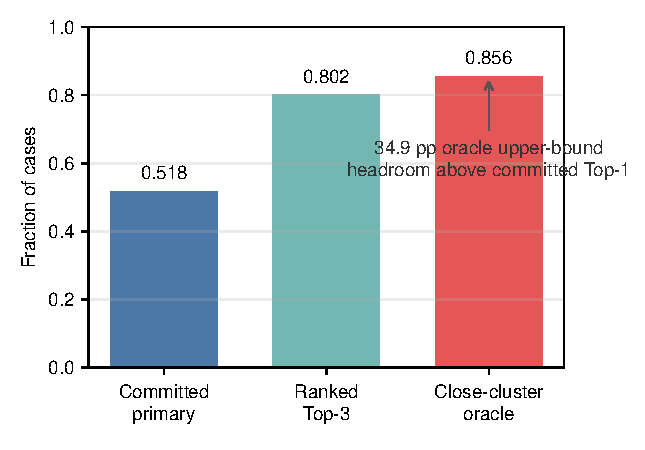
\includegraphics[width=0.98\textwidth]{fig_b_selection_bottleneck.pdf}
\caption{Committed Top-1 agreement and genuine Top-3 gold-label coverage on the 1,000-case internal held-out set. A benchmark gold parent appears in the genuine Top-3 in 802 cases but is selected as the committed primary diagnosis in 518 cases.}
\label{fig:selection-bottleneck}
\end{figure}

\paragraph{Criterion-compatible set.}
\label{sec:criterion-checking}
Among the 915 checker-eligible cases, the criterion-compatible set contains at least one benchmark gold parent in 857 cases, corresponding to 93.7\% inclusion (95\% CI [91.9\%, 95.1\%]). The median compatible set contains six of the fourteen configured diagnostic categories. The criterion path therefore has high gold-label inclusion but limited selectivity: it often retains the benchmark label together with several alternatives rather than identifying one preferred primary diagnosis.

\paragraph{Joint recorded-output profiles.}
Table~\ref{tab:d3rs-joint} reports the joint distribution of Top-3 candidate detection ($D_3$), gold-label inclusion in the criterion-compatible set ($I$), and committed-primary agreement ($S$) among the 915 checker-eligible cases.

\begin{table}[htbp]
\centering
\caption{Joint distribution of Top-3 candidate detection ($D_3$), gold-label inclusion in the criterion-compatible set ($I$), and committed-primary agreement ($S$) on the 915 checker-eligible cases.}
\label{tab:d3rs-joint}
\small
\setlength{\tabcolsep}{3pt}
\renewcommand{\arraystretch}{1.08}
\begin{tabularx}{\textwidth}{|>{\centering\arraybackslash}p{2.3cm}|>{\centering\arraybackslash}p{2.9cm}|>{\centering\arraybackslash}p{2.5cm}|>{\centering\arraybackslash}p{2.1cm}|X|}
\hline
Gold label in genuine Top-3 ($D_3$)? & Gold label in criterion-compatible set ($I$)? & Committed-primary agreement ($S$)? & Cases, $n$ (\%) & Interpretation\\
\hline
No & No & No & 34 (3.7\%) & Gold label absent from both views\\
\hline
No & Yes & No & 79 (8.6\%) & Compatible-set inclusion outside the Top-3\\
\hline
Yes & No & No & 12 (1.3\%) & Ranked; absent from compatible set\\
\hline
Yes & No & Yes & 12 (1.3\%) & Agreement; absent from compatible set\\
\hline
Yes & Yes & No & 272 (29.7\%) & Ranked and compatible; not selected\\
\hline
Yes & Yes & Yes & 506 (55.3\%) & Ranked, compatible, and selected\\
\hline
\end{tabularx}
\renewcommand{\arraystretch}{1.0}
\parbox{0.96\textwidth}{\footnotesize
\textit{Note.} Profiles with $D_3=0$ and $S=1$ are impossible under the DA ranking contract and are omitted. Percentages are shares of the 915 checker-eligible cases and may not sum to exactly 100\% because of rounding.
}
\end{table}

\ThesisFigure[0.98\textwidth]{fig_d3rs_flow.pdf}{Four mutually exclusive disagreement-localization groups among the 915 checker-eligible internal cases. Cases are first assigned by committed-primary agreement ($S$); cases with $S=0$ are then divided by Top-3 candidate detection ($D_3$) and gold-label inclusion ($I$). This analytical assignment order is not a runtime sequence.}{fig:d3rs-flow}

The six profiles in Table~\ref{tab:d3rs-joint} form the four analytical groups defined in Chapter~\ref{ch:experimental}: 518 cases with committed-primary agreement, 113 Top-3 candidate misses, 12 cases in which a gold parent is ranked but absent from the compatible set and not selected, and 272 cases in which a gold parent is ranked and compatible but not selected. The 79 cases with $D_3=0$ and $I=1$ are possible because all configured categories are checked, not only the Diagnostician's Top-3.

Among the 802 checker-eligible cases with a benchmark gold parent in the genuine Top-3, 778 (97.0\%) also contain a gold parent in the criterion-compatible set. Of these 778 cases, 506 (65.0\%) commit a gold parent as primary and 272 (35.0\%) commit another diagnosis. The 272-case group is therefore the largest recorded disagreement group after the candidate and compatibility outputs are considered.

This localization does not prove that the finalizer alone caused the disagreement. The ranking, criterion states, compatible set, and committed diagnosis are connected model-derived outputs, and the criterion-compatible set is not a ranked recommendation of the primary diagnosis. The result shows where disagreement is recorded, not the hidden causal mechanism that produced it.

\paragraph{Supplementary gold-informed oracle.}
Table~\ref{tab:oracle-headroom} reports the non-deployable oracle analysis defined in Section~\ref{sec:oracle-design}. The oracle directly uses benchmark labels and assumes that every eligible disagreement can be corrected without introducing a new error.

\begin{table}[htbp]
\centering
\caption{Gold-informed oracle estimate of primary-selection headroom on the internal held-out set ($N=1000$).}
\label{tab:oracle-headroom}
\small
\begin{tabularx}{\textwidth}{|>{\raggedright\arraybackslash}p{4.1cm}|c|c|X|}
\hline
Quantity & Cases & Rate & Interpretation\\
\hline
Observed committed-primary agreement & 518 & 0.518 & Cases with $S=1$ before oracle correction\\
\hline
Oracle-eligible disagreements & 349 & 0.349 & Initially disagreeing cases with a benchmark gold parent in a close supported cluster\\
\hline
Optimistic agreement under the no-harm assumption & 867 & 0.867 & The 518 observed agreements plus all 349 oracle-eligible disagreements\\
\hline
\end{tabularx}
\end{table}

Under these assumptions, the upper-bound agreement is $(518+349)/1000=0.867$. The 349 oracle-eligible cases follow the oracle's own candidate and support rules and are not the same quantity as the observed 272-case $D_3=1$, $I=1$, $S=0$ profile. The oracle demonstrates that the recorded outputs contain optimistic headroom; it does not provide a deployable selector or an expected performance estimate.

\paragraph{Answer to RQ2.}
Benchmark disagreement is observed at more than one output view, but the largest checker-eligible disagreement group occurs when a benchmark gold parent is already present in both the genuine Top-3 and the criterion-compatible set and another diagnosis is committed as primary. This pattern supports primary-selection analysis, while the broad compatible sets and causal limits prevent interpreting it as proof that one finalization component is the sole source of error.

\section{Primary-Selection Intervention Results}
\label{sec:nts-factorial}
\label{sec:additional-selection-results}

This section answers RQ4 with Direct-Answer (DA) as the reference and committed Top-1 Accuracy as the common outcome. Fixed-artifact policy comparisons are separated from methods that re-execute model stages or add repeated sampling.

\paragraph{Matched DA--NtS comparison.}
Table~\ref{tab:nts-factorial} compares DA with Nominate-then-Select (NtS) under no retrieval, global Top-5 retrieval, and parent-balanced retrieval. Within each condition, the two policies reuse the same Diagnostician ranking, criterion states, and criterion-compatible set. The reported difference is NtS minus DA.

\begin{table}[htbp]
\centering
\caption{Paired comparison of Direct-Answer (DA) and Nominate-then-Select (NtS) under three retrieval conditions on the internal held-out split ($N=1000$ per condition). Confidence intervals are paired-bootstrap intervals; negative differences favor DA.}
\label{tab:nts-factorial}
\small
\begin{tabular}{|l|c|c|c|}
\hline
Retrieval condition & DA Top-1 & NtS Top-1 & Difference (95\% CI), pp\\
\hline
No retrieval & 51.0\% & 48.2\% & $-2.8$ [$-4.1$, $-1.5$]\\
\hline
Global Top-5 & 52.4\% & 49.5\% & $-2.9$ [$-4.4$, $-1.4$]\\
\hline
Parent-balanced & 51.8\% & 49.0\% & $-2.8$ [$-4.3$, $-1.3$]\\
\hline
\end{tabular}
\end{table}

NtS reduces committed Top-1 by 2.8--2.9 percentage points in all three retrieval conditions, and each paired-bootstrap confidence interval excludes zero. The detailed discordant counts in Appendix~\ref{app:supporting} show more cases correct only under DA than cases correct only under NtS in every condition. The reduction is therefore not explained by one retrieval setting. The interaction contrasts are small and statistically inconclusive.

Because DA and NtS share the same upstream artifacts, this is the clearest test of finalization policy alone. The result shows that replacing the Diagnostician's proposed primary with the highest-ranked diagnosis selected by the evaluated NtS rule does not improve benchmark agreement. Under the evaluated rule, high gold-label inclusion in a compatible set with a median size of six is not sufficiently selective for reliable primary re-selection.

\paragraph{Additional primary-selection methods.}
Table~\ref{tab:internal-selection-results} summarizes the remaining internal methods relative to the validation-selected parent-balanced DA configuration.

\begin{table}[htbp]
\centering
\caption{Additional internal primary-selection methods relative to DA. Confidence intervals are paired-bootstrap intervals for the Top-1 difference; a dash denotes unavailable paired records.}
\label{tab:internal-selection-results}
\small
\renewcommand{\arraystretch}{1.08}
\begin{tabularx}{\textwidth}{|>{\raggedright\arraybackslash}p{3.2cm}|c|c|c|X|}
\hline
Method & Top-1 & $\Delta$ vs DA & 95\% CI & Interpretation\\
\hline
DA & 0.518 & --- & --- & Reference output\\
\hline
Deterministic fusion & 0.514 & $-0.004$ & --- & Recorded-output summary\\
\hline
Pairwise independent & 0.524 & $+0.006$ & [$-0.010$, 0.022] & Complete configuration\\
\hline
Two-view debate & 0.485 & $-0.033$ & [$-0.049$, $-0.018$] & Complete configuration\\
\hline
\end{tabularx}
\renewcommand{\arraystretch}{1.0}
\end{table}

Deterministic fusion is 0.4 percentage points below DA, but a complete paired case-level record was not retained, so no interval or case-level transition analysis is reported. Independent pairwise comparison is 0.6 percentage points above DA, but its confidence interval includes zero. It also comes from a separate full-pipeline execution, so the difference cannot be attributed only to the pairwise selector. Two-view debate is 3.3 percentage points below DA, and its confidence interval excludes zero. Internal self-consistency and confidence-informed self-consistency remain descriptive because only summary-level records were retained.

\paragraph{Answer to RQ4.}
None of the evaluated methods provides a clear and attributable improvement over DA on the internal held-out set. The matched NtS comparison consistently lowers Top-1, deterministic fusion is slightly lower without retained paired records, the small independent-pairwise increase is statistically inconclusive and confounded by a complete rerun, and debate performs below DA. The observed candidate and compatibility headroom therefore was not converted into a reliable gain by the tested selectors.

\section{Model-Scale and Diagnostic Disagreement Analysis}
\label{sec:model-scale-disagreement}

This section reports the internal model-scale and diagnostic-confusion results that contribute to RQ5. External synthetic transfer, diagnostic-scope expansion, and lexical transfer are reported in Chapter~\ref{ch:external}.

\paragraph{Model scale.}
\ThesisFigure{fig_a_size_robustness.pdf}{Held-out Top-1 across Qwen3 model sizes for the Single baseline and HiED--DA. Shaded bands indicate the observed minimum-to-maximum range across the evaluated model sizes and are not confidence intervals.}{fig:size-robustness}

Single Top-1 increases monotonically from 0.143 at 4B to 0.465 at 32B. HiED--DA Top-1 varies from 0.497 to 0.538 without a monotonic size trend, and its genuine Top-3 Accuracy remains between 0.803 and 0.818. These ranges are narrower than the change observed for Single, but they do not establish model-size invariance. They apply only to the evaluated Qwen3 family and fixed study settings.

The smallest-model runs also contained additional structured-output failures. These execution issues are not diagnostic outcomes. Exact counts and run-integrity notes are reported in Appendix~\ref{app:supporting}, Table~\ref{tab:qwen-size-results}.

\paragraph{Diagnostic confusion.}
The first-listed-label confusion analysis has agreement 0.509, compared with the any-gold committed Top-1 Accuracy of 0.518. The difference occurs because the confusion matrix assigns one first-listed projected benchmark parent to each case, whereas the main Top-1 measure counts a match with any projected benchmark gold parent.

\ThesisFigure{fig_d_confusion_heatmap.pdf}{Confusion matrix on the internal held-out set using the first-listed gold parent for each case.}{fig:confusion-thesis-rewrite}

The largest direction is F41$\rightarrow$F32 with 178 cases, compared with 24 cases in the reverse F32$\rightarrow$F41 direction. Other frequent directions are F39$\rightarrow$F32 (43), \emph{Others}$\rightarrow$F32 (37), and \emph{Others}$\rightarrow$F41 (26). These counts show that the disagreements are not distributed symmetrically and that F32 is a frequent destination. Because the matrix uses one first-listed benchmark label, it is descriptive rather than the primary multilabel evaluation. Chapter~\ref{ch:error} examines the candidate ranks, selection pairs, and criterion-state patterns behind these directions.

\paragraph{Internal contribution to RQ5.}
Within the evaluated Qwen3 family, HiED's ranked Top-3 coverage changes little across model sizes, while committed Top-1 varies over a narrower range than the Single baseline. The internal disagreements are also concentrated in a small number of diagnostic directions, especially F41$\rightarrow$F32. These findings define the internal boundary conditions; Chapter~\ref{ch:external} tests whether the broader stage-wise pattern persists under a second synthetic corpus and other diagnostic settings.

\section{Chapter Summary}

The internal results give five main answers. Retrieval improves the Single baseline more clearly than HiED, and parent-balanced retrieval remains the primary HiED configuration because of the validation contract rather than the held-out ranking. Single and HiED have almost identical committed Top-1 performance on Route B; no retained TF--IDF output covers that split, so no same-split lexical-superiority claim is made. The separate public-validation TF--IDF audit shows substantial same-source lexical predictability but is kept outside the Route B table. HiED nevertheless exposes a large difference between candidate availability, criterion compatibility, and committed-primary agreement: 272 of 915 checker-eligible cases contain a benchmark gold parent in both the Top-3 and compatible set but commit another diagnosis. The tested primary-selection interventions do not provide a clear attributable improvement over DA. Finally, HiED's Top-3 coverage is comparatively stable across the evaluated Qwen3 sizes, while the remaining disagreements are concentrated toward a small number of diagnostic directions. Chapter~\ref{ch:external} examines whether these patterns persist under external synthetic distribution shift.

\chapter{External Synthetic Evaluation}
\label{ch:external}

This chapter examines whether the main recorded-output patterns remain visible when HiED is applied to a second synthetic Chinese dialogue corpus. The external corpus is MDD-5k. It was produced through a different data-generation process from LingxiDiag and therefore provides a cross-corpus boundary test. It does not provide real-patient or prospective clinical validation.

The frozen repository contains several MDD-5k result lineages. They were created for different purposes and do not contain identical case outputs. This chapter therefore keeps three questions separate:

\begin{enumerate}
    \item How does one matched 925-case HiED trace perform under the thesis-wide any-gold scoring contract?
    \item Do the same \(D_3\), \(I\), and \(S\) output profiles remain observable on its 878 checker-eligible cases?
    \item How do alternative primary-selection methods compare when they reuse or extend that matched trace?
\end{enumerate}

A separate canonical-rescore trace is reported only as a sensitivity analysis. It is not merged with the matched method-comparison trace.

\section{External Populations and Trace Lineages}
\label{sec:external-populations}

Table~\ref{tab:external-inventory} summarizes the external populations and their roles.

\begin{table}[htbp]
\centering
\caption{External MDD-5k populations and evidence lineages used in this chapter.}
\label{tab:external-inventory}
\small
\begin{tabularx}{\textwidth}{|>{\raggedright\arraybackslash}p{3.5cm}|c|>{\raggedright\arraybackslash}X|}
\hline
\textbf{Population or lineage} & \textbf{Cases} & \textbf{Role and boundary}\\
\hline
Matched method-comparison trace, all cases & 925 & Main external HiED result and common source for the selector comparisons in Section~\ref{sec:mdd-multiway}.\\
\hline
Matched method-comparison trace, checker-eligible cases & 878 & Cases with at least one benchmark gold diagnosis represented by the configured non-\emph{Others} checker scope. Used for \(D_3\), \(I\), and \(S\).\\
\hline
Canonical-rescore trace & 925 total; 878 checker-eligible & Separately archived trace rescored under the thesis-wide any-gold contract. Used only to show trace sensitivity; not combined with the matched method-comparison trace.\\
\hline
F32--F41 binary subset & 490 & Narrow scope-restricted sensitivity population retained in the archived rescore material. It is not used for the main multiway stage-wise claim.\\
\hline
\end{tabularx}
\end{table}

The main results below use one matched 925-case method-comparison trace. For every case, the benchmark gold diagnoses, committed primary diagnosis, Diagnostician ranking, and criterion-compatible set come from the same recorded output. All labels are projected to the paper parent space. A case is counted as correct when the committed primary matches any projected benchmark gold parent, following the metric contract in Chapter~\ref{ch:data}.

This distinction matters because older external summaries mixed values from different traces or used the first listed gold diagnosis instead of the complete projected gold set. The recalculation used here does not combine those contracts.

\section{Main External Performance}
\label{sec:external-main-performance}

Table~\ref{tab:external-summary-rewrite} compares the validation-selected internal HiED--DA result with the matched external trace. The internal and external rows are descriptive results from different synthetic corpora; they are not paired observations.

\begin{table}[htbp]
\centering
\caption{Internal and external HiED--DA results under the thesis-wide any-gold contract. External values come from one matched method-comparison trace.}
\label{tab:external-summary-rewrite}
\small
\begin{adjustbox}{max width=\textwidth}
\begin{tabular}{|l|c|c|c|c|c|}
\hline
\textbf{Population} & \textbf{Cases} & \textbf{Top-1} & \shortstack{\textbf{Genuine}\\\textbf{Top-3}} & \shortstack{\textbf{Gold in}\\\textbf{compatible set}} & \shortstack{\textbf{Median compatible-}\\\textbf{set size}}\\
\hline
LingxiDiag internal held-out & 1,000 & 0.518 & 0.802 & 0.937$^{*}$ & 6\\
\hline
MDD-5k, all cases & 925 & 0.571 & 0.851 & --- & ---\\
\hline
MDD-5k, checker-eligible & 878 & 0.601 & 0.896 & 0.786 & 6\\
\hline
\end{tabular}
\end{adjustbox}
\parbox{0.96\textwidth}{\footnotesize
\textit{Note.} $^{*}$The internal compatibility value uses the 915 checker-eligible LingxiDiag cases rather than all 1,000 cases. MDD-5k compatibility is reported only for the 878 checker-eligible cases.}
\end{table}

On all 925 MDD-5k cases, HiED--DA commits a benchmark-consistent primary diagnosis in 528 cases, giving Top-1 Accuracy of 0.571. A benchmark gold parent appears in the genuine Top-3 in 787 cases, giving Top-3 Accuracy of 0.851.

The 47 cases outside the configured checker scope cannot contribute a gold-parent criterion-inclusion result. After these cases are removed, the same 528 committed-primary agreements give Top-1 Accuracy of 0.601 on 878 cases. Genuine Top-3 coverage is 787 of 878, or 0.896. The criterion-compatible set contains at least one benchmark gold parent in 690 cases, or 0.786, and its median parent-collapsed size is six.

The external result therefore does not show that criterion inclusion remains unchanged across corpora. Candidate coverage is high, but compatibility inclusion is lower than in the internal analysis. The main transferable observation is narrower: candidate availability, compatibility, and primary commitment remain measurably different output views.

Figure~\ref{fig:internal-external-gap} compares the three recorded views on the internal and external checker-eligible populations.

\begin{figure}[htbp]
\centering
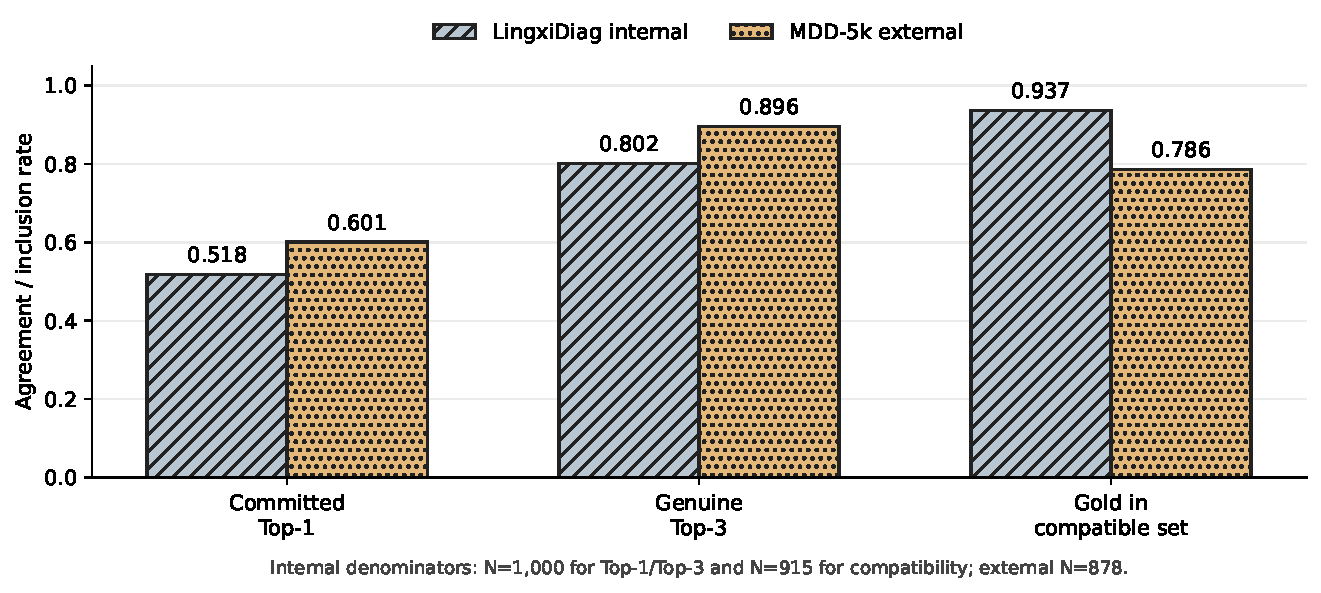
\includegraphics[width=0.9\textwidth]{fig_internal_external_gap.pdf}
\caption{Committed Top-1 agreement, genuine Top-3 coverage, and benchmark-gold inclusion in the criterion-compatible set for the internal and matched external traces. The denominators differ: internal Top-1 and Top-3 use 1,000 cases, internal compatibility uses 915 checker-eligible cases, and all three external values use the stated 878-case checker-eligible population except the all-case external headline reported separately in Table~\ref{tab:external-summary-rewrite}.}
\label{fig:internal-external-gap}
\end{figure}
\FloatBarrier
\section{External Recorded-Output Profiles}
\label{sec:external-stagewise}

Table~\ref{tab:external-disagreement-profiles} reports the complete joint distribution of genuine Top-3 detection (\(D_3\)), benchmark-gold inclusion in the criterion-compatible set (\(I\)), and committed-primary agreement (\(S\)) on the 878 checker-eligible cases.

\begin{table}[htbp]
\centering
\caption{Joint distribution of \(D_3\), \(I\), and \(S\) on the matched 878-case external trace.}
\label{tab:external-disagreement-profiles}
\small
\setlength{\tabcolsep}{4pt}
\begin{tabularx}{\textwidth}{|c|c|c|r|>{\raggedright\arraybackslash}X|}
\hline
\(\boldsymbol{D_3}\) & \(\boldsymbol{I}\) & \(\boldsymbol{S}\) & \textbf{Cases, \(n\) (\%)} & \textbf{Recorded-output profile}\\
\hline
0 & 0 & 0 & 20 (2.3\%) & Gold parent absent from both the genuine Top-3 and compatible set\\
\hline
0 & 1 & 0 & 71 (8.1\%) & Gold parent appears in the compatible set but not in the genuine Top-3\\
\hline
1 & 0 & 0 & 34 (3.9\%) & Gold parent is ranked but absent from the compatible set, and another primary is committed\\
\hline
1 & 0 & 1 & 134 (15.3\%) & A benchmark-consistent primary is committed even though the gold parent is absent from the compatible set\\
\hline
1 & 1 & 0 & 225 (25.6\%) & Gold parent is ranked and compatible but is not committed as primary\\
\hline
1 & 1 & 1 & 394 (44.9\%) & Gold parent is ranked, compatible, and committed\\
\hline
\end{tabularx}
\parbox{0.96\textwidth}{\footnotesize
\textit{Note.} The table uses one matched trace and the complete projected gold-label set. Rows with \(D_3=0\) and \(S=1\) do not occur under the recorded DA ranking contract. Percentages may not sum to exactly 100\% because of rounding.}
\end{table}

The 878 cases can also be summarized into four mutually exclusive outcome groups:

\begin{itemize}
    \item 528 cases (60.1\%) have committed-primary agreement;
    \item 91 cases (10.4\%) disagree and contain no benchmark gold parent in the genuine Top-3;
    \item 34 cases (3.9\%) disagree after the gold parent is ranked but remains absent from the compatible set; and
    \item 225 cases (25.6\%) contain a benchmark gold parent in both the genuine Top-3 and compatible set but commit another diagnosis.
\end{itemize}

The last group is the largest recorded disagreement profile, so a primary-selection difference remains visible on the second synthetic corpus. However, the full joint table also shows an important limitation: 134 benchmark-consistent committed primaries occur even though the corresponding gold parent is absent from the compatible set. Criterion compatibility is therefore neither necessary nor sufficient for the DA commitment in this trace.

A benchmark gold parent appears in both the genuine Top-3 and compatible set in 619 cases. Of these, 394 commit a benchmark-consistent primary, or 63.7\%. The remaining 225 cases form the ranked-and-compatible nonselection group. This result localizes a recorded disagreement; it does not prove that the finalizer alone caused it.

\section{Matched Primary-Selection Comparisons}
\label{sec:mdd-multiway}

The primary-selection comparisons in this section use the same 925-case variant battery. Direct-Answer (DA) is the reference. The methods differ in what they reuse and whether they introduce new model inference, so the evidence contract is stated in the table.

\begin{table}[htbp]
\centering
\caption{External primary-selection methods on the common 925-case matched trace. Differences and confidence intervals are relative to DA.}
\label{tab:mdd-finalization-results}
\small
\begin{tabularx}{\textwidth}{|>{\raggedright\arraybackslash}p{3.3cm}|>{\raggedright\arraybackslash}p{4.5cm}|c|c|}
\hline
\textbf{Method} & \textbf{Evidence contract} & \textbf{Top-1} & \(\boldsymbol{\Delta}\) \textbf{vs DA, pp (95\% CI)}\\
\hline
Direct-Answer & Reference committed primary & 57.08\% & ---\\
\hline
Nominate-then-Select & Same upstream trace; deterministic compatibility-based re-selection & 40.65\% & \(-16.43\) [\(-19.5\), \(-13.5\)]\\
\hline
Deterministic fusion & Same upstream trace; deterministic fusion of recorded outputs & 47.14\% & \(-9.95\) [\(-12.4\), \(-7.5\)]\\
\hline
Posthoc fixed-trace forced-commit sweep & Reuses saved pairwise preferences; not an independently rerun system & 54.59\% & \(-2.49\) [\(-4.1\), \(-1.1\)]\\
\hline
Independent pairwise & Separate full-pipeline configuration & 57.08\% & \(0.00\) [0.0, 0.0]\\
\hline
Two-view debate & Separate full-pipeline configuration & 37.84\% & \(-19.24\) [\(-22.1\), \(-16.4\)]\\
\hline
Self-consistency, \(K=3\) & Repeated-generation summary record & 57.84\% & \(+0.76\) [\(-0.5\), 2.1]\\
\hline
Self-consistency, \(K=5\) & Repeated-generation summary record & 58.16\% & \(+1.08\) [\(-0.1\), 2.4]\\
\hline
Confidence-informed SC, \(K=3\) & Repeated-generation summary record & 57.84\% & \(+0.76\) [\(-0.5\), 2.1]\\
\hline
Confidence-informed SC, \(K=5\) & Repeated-generation summary record & 58.16\% & \(+1.08\) [\(-0.1\), 2.4]\\
\hline
\end{tabularx}
\end{table}

NtS and deterministic fusion both reduce committed Top-1 agreement. This is consistent with the joint profile table: the criterion-compatible set omits a benchmark gold parent in 168 cases whose gold parent is nevertheless ranked, including 134 cases that DA commits correctly. Replacing the proposed primary with a compatibility-based choice can therefore overturn benchmark-consistent decisions as well as disagreements.

The posthoc forced-commit sweep also lowers Top-1. Its name describes the replay rule, not an independently executed pairwise system. It promotes preferences already stored in the matched pairwise trace and should be interpreted only as a fixed-trace policy sensitivity.

Independent pairwise produces the same committed Top-1 as DA. The comparison stage was active, but under this output contract it reordered candidates without replacing the committed primary. Two-view debate lowers agreement. Self-consistency and confidence-informed self-consistency have small positive point estimates, but their intervals include zero and only summary-level records are retained. None of the evaluated methods therefore provides a clear and attributable external improvement over DA.

Detailed discordant counts and exact McNemar tests are reported in Appendix~\ref{app:supporting}, Table~\ref{tab:external-paired-tests}.

\section{Trace-Lineage and Diagnostic-Scope Boundaries}
\label{sec:external-lineage-sensitivity}

The matched method-comparison trace is not the only archived MDD-5k output. Table~\ref{tab:external-trace-sensitivity} shows how the same any-gold recalculation changes when it is applied to a separately archived canonical-rescore trace.

\begin{table}[htbp]
\centering
\caption{Sensitivity of external results to the archived trace lineage under the same any-gold scoring contract.}
\label{tab:external-trace-sensitivity}
\label{tab:scope-expansion-results}
\small
\begin{tabularx}{\textwidth}{|>{\raggedright\arraybackslash}p{4.1cm}|c|c|c|c|}
\hline
\textbf{Trace and population} & \textbf{Cases} & \textbf{Top-1} & \textbf{Genuine Top-3} & \textbf{Gold in compatible set}\\
\hline
Matched method-comparison, all cases & 925 & 0.571 & 0.851 & ---\\
\hline
Canonical rescore, all cases & 925 & 0.587 & 0.857 & ---\\
\hline
Matched method-comparison, checker-eligible & 878 & 0.601 & 0.896 & 0.786\\
\hline
Canonical rescore, checker-eligible & 878 & 0.618 & 0.903 & 0.959\\
\hline
\end{tabularx}
\end{table}

The two traces have the same nominal case counts but different stored outputs. Their Top-1 values differ by 1.6 percentage points, and their criterion-inclusion rates differ much more. This sensitivity is why the chapter does not combine a primary diagnosis from one trace with the ranking or compatibility set from another.

A previously cited F60 scope-expansion result could not be linked to a preserved source artifact in the frozen repository snapshot. Its numerical values are therefore not reported in this revision. The underlying methodological point remains: a diagnosis cannot be recovered if it is absent from the configured output space, but expanding that space does not by itself establish accurate selection.

\section{Cross-Corpus Lexical Transfer}
\label{sec:external-lexical-transfer}

The lexical transfer analysis uses a separately preserved full-corpus TF--IDF with logistic-regression matrix. Its LingxiDiag evaluation population is the public-validation split rather than Route B. Table~\ref{tab:lexical-transfer-rewrite} reports Top-1 and genuine Top-3 values under that artifact's twelve-class parent-label contract.

\begin{table}[htbp]
\centering
\caption{Full-corpus cross-source transfer of TF--IDF with logistic regression.}
\label{tab:lexical-transfer-rewrite}
\small
\begin{tabularx}{\textwidth}{|>{\raggedright\arraybackslash}p{3.3cm}|>{\raggedright\arraybackslash}p{3.3cm}|c|c|c|}
\hline
\textbf{Training source} & \textbf{Evaluation source} & \textbf{Cases} & \textbf{Top-1} & \textbf{Top-3}\\
\hline
LingxiDiag-16K & LingxiDiag public validation & 1,000 & 0.602 & 0.935\\
\hline
LingxiDiag-16K & MDD-5k & 925 & 0.059 & 0.613\\
\hline
MDD-5k & MDD-5k & 925 & 0.632 & 0.842\\
\hline
MDD-5k & LingxiDiag public validation & 1,000 & 0.476 & 0.676\\
\hline
\end{tabularx}
\parbox{0.96\textwidth}{\footnotesize
\textit{Note.} These are full-corpus transfer runs. The LingxiDiag evaluation rows use the public-validation split, not the Route B internal held-out set. They are not the previously reported F32--F41 subset values and should not be interpreted as that binary experiment.}
\end{table}

The classifier is strongest when training and evaluation use the same corpus. Training on LingxiDiag and testing on MDD-5k reduces Top-1 from 0.602 to 0.059. The reverse transfer is less severe but still lower than within-MDD evaluation: 0.476 instead of 0.632. The asymmetric drop shows that lexical regularities and label distributions differ across the two synthetic generation processes.

This result does not show that an LLM architecture automatically generalizes clinically. It shows that a strong same-corpus lexical score should not be treated as evidence of source-independent diagnosis performance.

\section{Answer to RQ5 and Chapter Summary}

\paragraph{Answer to RQ5.}
The stage-wise output pattern remains observable on MDD-5k, but it is not identical to the internal pattern. In the matched 878-case external trace, 225 cases (25.6\%) contain a benchmark gold parent in both the genuine Top-3 and the criterion-compatible set but commit another diagnosis as primary. This is the largest recorded disagreement profile. At the same time, external compatibility inclusion is lower than the internal value, and the exact rates change across archived trace lineages. The external evidence therefore supports the portability of the stage-wise analysis framework, not universal stability of the numerical results.

The matched selection experiments also reproduce the main negative finding: deterministic re-selection from the recorded compatibility outputs does not improve DA. Additional pairwise, debate, or repeated-generation configurations do not provide a clear and attributable improvement.

Finally, the lexical transfer matrix shows large source effects. Together, these results establish a synthetic cross-corpus boundary for the study. They do not establish real-patient validity, a uniquely correct clinical primary diagnosis, or improved clinical efficiency.

\chapter{Characterization of Recorded-Output Disagreements}
\label{ch:error}

This chapter describes where HiED disagrees with the projected benchmark labels in one frozen internal held-out trace. It does not estimate clinical diagnostic error. LingxiDiag contains synthetic dialogues, the benchmark labels are dataset references rather than independently adjudicated clinical diagnoses, and the saved outputs do not reveal the model's hidden reasoning.

The analysis asks three simple questions. Was a benchmark-reference diagnosis present in the genuine Top-3? Was it present in the criterion-compatible set? Was a benchmark-reference diagnosis committed as primary? Keeping these views separate shows where disagreement is recorded, but it does not prove that one stage caused another stage to fail.

\section{Analysis Population and Output Views}
\label{sec:ch8-stagewise-taxonomy}

The internal held-out set contains 1,000 cases. Criterion-level analysis is available for 915 cases with at least one non-\emph{Others} benchmark parent represented by a configured Criterion Checker. For these cases, Chapter~\ref{ch:results} defines:

\begin{itemize}
    \item $D_3=1$ when at least one benchmark-reference parent appears in the genuine Diagnostician Top-3;
    \item $I=1$ when at least one benchmark-reference parent appears in the criterion-compatible set; and
    \item $S=1$ when the committed primary diagnosis agrees with at least one benchmark-reference parent.
\end{itemize}

Table~\ref{tab:ch8-joint-profiles} repeats the complete joint distribution because the six profiles are the basis of this chapter.

\begin{table}[htbp]
\centering
\caption{Recorded $D_3/I/S$ profiles among the 915 checker-eligible internal cases.}
\label{tab:ch8-joint-profiles}
\small
\begin{tabularx}{\textwidth}{|c|c|c|r|X|}
\hline
$D_3$ & $I$ & $S$ & Cases & Recorded interpretation\\
\hline
0 & 0 & 0 & 34 & Reference absent from both recorded upstream views\\
\hline
0 & 1 & 0 & 79 & Reference absent from Top-3 but present in compatible set\\
\hline
1 & 0 & 0 & 12 & Reference ranked, absent from compatible set, and not selected\\
\hline
1 & 0 & 1 & 12 & Benchmark-consistent primary despite compatibility absence\\
\hline
1 & 1 & 0 & 272 & Reference ranked and compatible but not selected\\
\hline
1 & 1 & 1 & 506 & Reference ranked, compatible, and selected\\
\hline
\end{tabularx}
\end{table}

The largest benchmark-disagreement profile is the 272-case group with $D_3=1$, $I=1$, and $S=0$. A benchmark-reference diagnosis is visible in both recorded upstream views, but another diagnosis is committed as primary. This is the strongest recorded profile of a primary-commitment disagreement under the tested HiED setting. It is not proof that finalization is a universal clinical bottleneck or the only cause of the disagreement.

The table also shows that compatibility is neither sufficient nor necessary for benchmark-consistent commitment in this trace. There are 272 cases in which a benchmark-reference diagnosis is compatible but not committed, and 12 cases in which a benchmark-consistent primary is committed even though the reference diagnosis is absent from the compatible set.

The 349-case gold-informed oracle population reported in Chapter~\ref{ch:results} is not an observed system group. It uses benchmark labels to define optimistic recoverability and is intentionally non-deployable. This chapter therefore describes only the outputs that the frozen system actually recorded.

\section{Candidate and Compatibility Disagreement Profiles}

Across all 1,000 internal cases, 198 contain no benchmark-reference parent in the genuine Top-3. Of these, 113 are checker-eligible and 85 are scored as the evaluation-only \emph{Others} category. Among the 113 checker-eligible Top-3 misses, 79 still contain a benchmark-reference parent in the criterion-compatible set, while 34 contain it in neither recorded view.

A separate group of 24 checker-eligible cases contains a benchmark-reference parent in the genuine Top-3 but not in the criterion-compatible set. Twelve of these cases still commit a benchmark-consistent primary diagnosis, while 12 do not. Because the disagreement subgroup contains only 12 cases, its criterion-state pattern is treated as descriptive rather than stable evidence about a general failure mode.

These results follow directly from the non-nested architecture. Criterion Checkers evaluate all configured categories rather than only the Diagnostician Top-3. A diagnosis can therefore be absent from the Top-3 but present in the compatible set, or ranked and committed even when its checker output does not place it in that set.

\section{Ranked and Criterion-Compatible but Not Selected}
\label{sec:ch8-primary-selection}

The 272-case group is examined in more detail because it is the largest recorded benchmark-disagreement profile. Figure~\ref{fig:ch8-reference-rank} shows the position of the highest-ranked benchmark-reference parent.

\ThesisFigure[0.72\textwidth]{fig_ch8_reference_rank.pdf}{Rank of the highest-ranked benchmark-reference parent among the 272 cases with $D_3=1$, $I=1$, and $S=0$.}{fig:ch8-reference-rank}
\FloatBarrier

The benchmark-reference parent is ranked second in 171 cases (62.9\%) and third in 101 cases (37.1\%). In most cases it is therefore the closest recorded alternative to the leading diagnosis, but rank proximity alone does not explain why another diagnosis is committed.

Table~\ref{tab:ch8-selection-pairs} reports the most frequent benchmark-reference-to-committed-primary directions.

\begin{table}[htbp]
\centering
\caption{Most frequent benchmark-reference-to-committed-primary pairs in the 272-case group.}
\label{tab:ch8-selection-pairs}
\small
\begin{tabularx}{\textwidth}{|>{\raggedright\arraybackslash}X|>{\raggedright\arraybackslash}p{3.2cm}|r|r|}
\hline
Highest-ranked benchmark-reference parent & Committed primary & Cases & Share\\
\hline
F41 & F32 & 158 & 58.1\%\\
F39 & F32 & 35 & 12.9\%\\
F32 & F41 & 11 & 4.0\%\\
F41 & F42 & 9 & 3.3\%\\
F51 & F32 & 9 & 3.3\%\\
\hline
\end{tabularx}
\parbox{0.96\textwidth}{\footnotesize
\textit{Note.} Each case contributes one pair based on its highest-ranked benchmark-reference parent. Percentages use the 272-case group as the denominator; only the five most frequent pairs are shown.}
\end{table}

The five pairs account for 222 cases (81.6\%), and F41-to-F32 alone accounts for 158 cases (58.1\%). These are directional benchmark disagreements under the paper's parent-label projection. They are not psychiatrist-confirmed misdiagnoses. Their concentration may reflect several factors, including class frequency, synthetic wording, overlapping symptom descriptions, parent-label projection, and model preference. The frozen trace cannot separate these causes.

\section{Diagnostic-Set Construction Disagreements}
\label{sec:ch8-diagnostic-set}

Committed-primary agreement does not guarantee agreement between the complete emitted diagnosis set and the benchmark-reference set. Among the 1,000 internal cases, HiED--DA commits a benchmark-consistent primary diagnosis in 518 cases. Exact set agreement occurs in 409 cases, leaving 109 cases with primary agreement but diagnostic-set disagreement.

\begin{table}[htbp]
\centering
\caption{Mutually exclusive diagnostic-set disagreement types among the 109 cases with benchmark-consistent committed primary diagnosis.}
\label{tab:ch8-diagnostic-set-errors}
\small
\begin{tabularx}{\textwidth}{|>{\raggedright\arraybackslash}X|r|r|}
\hline
\textbf{Diagnostic-set disagreement type} & \textbf{Cases} & \textbf{Share}\\
\hline
Additional emitted diagnosis only & 55 & 50.5\%\\
\hline
Omitted benchmark-reference diagnosis only & 52 & 47.7\%\\
\hline
Both additional and omitted diagnoses & 2 & 1.8\%\\
\hline
Total & 109 & 100.0\%\\
\hline
\end{tabularx}
\end{table}

The benchmark contains one projected parent in 912 cases, two in 83 cases, and three in five cases. An additional emitted diagnosis is counted as an addition because it is absent from that reference set; the benchmark does not establish that the added diagnosis is clinically false. These results show why Top-1, Exact Match, Macro-F1, and Weighted-F1 describe different parts of the output contract.

\section{Criterion-State Composition}
\label{sec:ch8-criterion-evidence}

The Criterion Checker records each item as \texttt{met}, \texttt{not\_met}, or \texttt{insufficient\_\allowbreak{}evidence}. Figure~\ref{fig:ch8-criterion-composition} compares mean within-case proportions across the four mutually exclusive analysis groups. Each case is summarized before group averaging so that cases with more recorded criterion items do not receive more weight. The corresponding medians and interquartile ranges are reported in Appendix~\ref{app:supporting}, Table~\ref{tab:ch8-criterion-ratios}.

\begin{figure}[htbp]
\centering
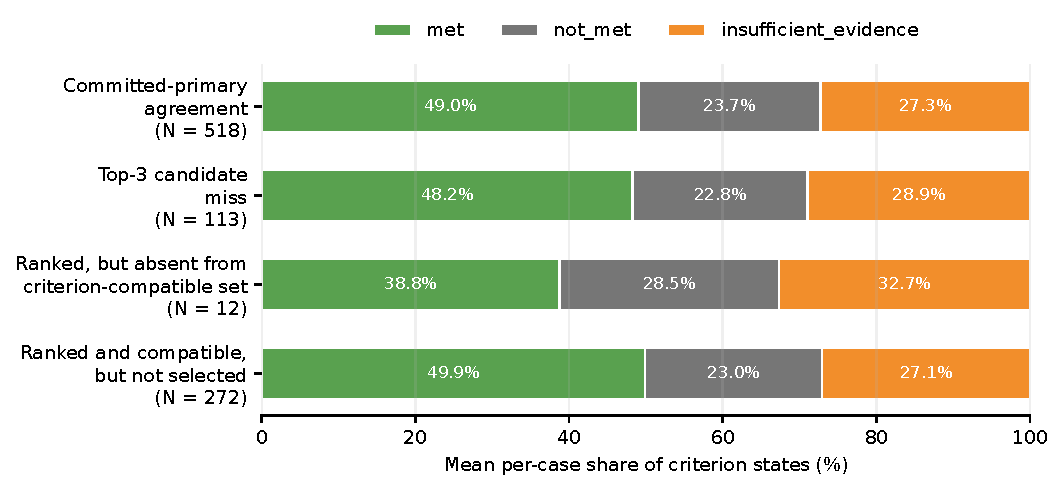
\includegraphics[width=1.0\textwidth]{fig_ch8_criterion_state_composition.pdf}
\caption{Mean within-case composition of recorded criterion states across the four mutually exclusive output groups among the 915 checker-eligible internal cases.}
\label{fig:ch8-criterion-composition}
\end{figure}
\FloatBarrier

The 272-case group and the committed-primary-agreement group have closely overlapping criterion-state compositions. Top-3 candidate misses are also broadly similar. The 12-case ranked-but-not-compatible disagreement group has fewer \texttt{met} states and more unresolved evidence on average, but its small size does not support a stable group-level conclusion.

Criterion checking makes the problem easier to inspect, but broad compatibility does not solve the final comparison. Compatible-set size and aggregate criterion-state proportions do not identify which compatible diagnosis will be committed as primary in this trace. These summaries are descriptive associations, not evidence that one criterion-state pattern caused the final commitment.

\section{Selected Frozen-Output Examples}
\label{sec:ch8-trace-boundaries}

Table~\ref{tab:audit-trace-examples} presents four deterministic examples from the same frozen internal trace. For each profile, the example is the first matching source record. No transcript text or checker evidence text is reproduced. The rows illustrate the meaning of the recorded profiles; they do not support population estimates or clinical conclusions.

\begingroup
\footnotesize
\setlength{\tabcolsep}{3pt}
\renewcommand{\arraystretch}{1.08}
\begin{longtable}{|>{\raggedright\arraybackslash}p{2.5cm}|>{\raggedright\arraybackslash}p{3.0cm}|>{\raggedright\arraybackslash}p{8.0cm}|}
\caption{Deterministically selected examples from four recorded $D_3/I/S$ profiles.}
\label{tab:audit-trace-examples}\\
\hline
Profile & Frozen record & Recorded outputs\\
\hline
\endfirsthead
\hline
Profile & Frozen record & Recorded outputs\\
\hline
\endhead
$D_3=0,I=0,S=0$ & Source line 6\newline Case \texttt{302945002} & Benchmark parent F31; Top-3 F32, F39, F41; compatible parents F43, F51, F32, F39, F98, F41; committed primary F32; no F31 criterion was marked \texttt{insufficient\_\allowbreak{}evidence}.\\
\hline
$D_3=1,I=0,S=0$ & Source line 26\newline Case \texttt{396572486} & Benchmark parent F32; Top-3 F39, F32, F41; compatible parents F51, Z71, F98; committed primary F39; F32 criteria B1, C2, C5, and C7 were marked \texttt{insufficient\_\allowbreak{}evidence}.\\
\hline
$D_3=1,I=0,S=1$ & Source line 46\newline Case \texttt{393127297} & Benchmark parent F32; Top-3 F32, F39, F51; compatible parents F51, F98, F39, F41; committed primary F32; all eleven recorded F32 criteria were marked \texttt{insufficient\_\allowbreak{}evidence}.\\
\hline
$D_3=1,I=1,S=0$ & Source line 25\newline Case \texttt{342807095} & Benchmark parent F32; Top-3 F20, F32, F41; compatible parents F43, F20, F32, F41, F39; committed primary F20; F32 criteria C2 and C7 were marked \texttt{insufficient\_\allowbreak{}evidence}.\\
\hline
\end{longtable}
\endgroup

The examples show why the recorded views must remain separate. Compatibility does not force selection, and compatibility absence does not prevent DA from keeping a benchmark-consistent proposed primary. Criterion IDs are study-rule identifiers, not independent clinical annotations. The examples also do not reveal why the language model produced its ranking or primary choice.

\section{Chapter Summary}
\label{sec:ch8-summary}

The largest internal benchmark-disagreement profile contains 272 cases in which a benchmark-reference diagnosis is present in both the genuine Top-3 and the criterion-compatible set but another diagnosis is committed as primary. The reference is usually ranked second, and several disagreement directions occur repeatedly. Diagnostic-set and criterion-state analyses add further detail, while the selected frozen examples show how the recorded views can disagree within one case.

These findings support the thesis claim that candidate generation, criterion checking, compatibility analysis, and primary commitment should be recorded and evaluated separately. They do not establish an overall accuracy advantage for HiED, a universal finalization bottleneck, a clinically validated confusion pattern, or a causal effect of criterion states. Those stronger conclusions require clinician adjudication or controlled experiments beyond the synthetic frozen-output analysis.

\chapter{Discussion}
\label{ch:discussion}

The results support a stage-wise interpretation of HiED rather than an accuracy-leading claim. Single and HiED have almost the same committed Top-1 result on Route B. A separate public-validation TF--IDF audit shows strong same-source lexical prediction, but no retained TF--IDF output covers Route B, so it is not treated as a same-split superiority result. HiED's distinct contribution is the set of recorded outputs that makes candidate generation, criterion checking, compatibility analysis, and primary commitment separately visible.

The internal and external analyses show the same broad type of benchmark disagreement: a reference diagnosis can be present in the ranked candidates and the criterion-compatible set, while another diagnosis is committed as primary. The size of this profile differs across datasets and archived traces. The framework for asking the stage-wise questions therefore transfers more clearly than the numerical rates themselves.

\section{Compatibility and Primary Selection in the Evaluated Trace}
\label{sec:discussion-primary-selection}

Candidate generation, criterion checking, and primary selection answer different questions. Candidate generation asks which diagnoses remain plausible. Criterion checking asks whether the fixed transcript supports each configured diagnosis under the study rules. Primary selection asks which diagnosis should be committed after comparing the plausible alternatives.

Common mental disorders share many symptoms. Poor sleep, fatigue, poor concentration, low mood, worry, avoidance, and reduced daily function may support several categories at the same time. A diagnosis can therefore pass its own compatibility rule without being the best primary explanation. It may instead be secondary, comorbid, less specific, or still uncertain.

Criterion checking makes this problem easier to inspect, but broad compatibility does not solve the final comparison. The internal compatible set contains a median of six configured categories, and its size and overall criterion-state composition do not clearly separate committed-primary agreement from the largest disagreement group. External results also show that compatibility is not a sufficient condition for selection and is not a necessary condition for a benchmark-consistent DA commitment.

The 272 internal cases and 225 external cases with a ranked and compatible reference diagnosis that is not selected are therefore best described as the largest recorded benchmark-disagreement profiles. They show that available upstream records do not automatically determine the final commitment. They do not prove that the finalizer alone caused the disagreement or that primary selection is the largest clinical difficulty in all settings.

A stronger primary selector would need direct comparisons among candidates. Useful information may include symptom timing, illness course, episode structure, syndrome dominance, exclusionary causes, explanatory dependence, and comorbidity. The current criterion path mainly checks diagnoses one at a time and does not fully represent these relations.

\section{Why the Tested Selection Methods Did Not Close the Gap}
\label{sec:discussion-selection-strategies}

DA versus NtS is the clearest matched finalization comparison because both policies reuse the same ranked candidates, criterion states, and criterion-compatible set. NtS lowers committed Top-1 under all three internal retrieval settings. A simple rule that prefers compatible candidates can correct some disagreements, but it can also replace an initially benchmark-consistent DA choice. This is expected when several diagnoses pass broad compatibility rules.

Deterministic fusion uses another fixed summary of the same records and also does not provide a clear gain. Pairwise comparison, debate, and repeated generation make the comparison more explicit, but they also add new prompts, model calls, context arrangements, or sampling budgets. Their results must therefore be read as complete-configuration results rather than isolated tests of one finalization component.

All tested methods use the same fixed transcript. More inference can reorganize the available evidence, but it cannot recover facts that were never recorded, such as symptom onset, previous episodes, exclusionary medical causes, or the relation between anxiety and mood symptoms. Sampling also measures preference stability rather than clinical validity. A model can repeat the same answer because it has a stable interpretation, or because it has a stable corpus prior or bias.

The observed Top-3--Top-1 gap is therefore decision headroom, not demonstrated automatic recoverability. The experiments show that the tested prompts, rules, and inference budgets did not reliably convert candidate availability into better committed-primary agreement. They do not show that every future comparative selector must fail.

\section{Boundaries Beyond Primary Selection}
\label{sec:discussion-set-scope-transfer}

Primary commitment is only one part of a diagnostic output. Diagnostic-set construction determines which additional diagnoses are emitted. Chapter~\ref{ch:error} shows 109 cases in which the committed primary agrees with the benchmark but the complete emitted set does not. This is why Top-1, Exact Match, Macro-F1, and Weighted-F1 must remain separate.

Diagnostic scope is another boundary. A diagnosis that is absent from the configured output space cannot be ranked or emitted. An earlier F60 scope-expansion result could not be linked to a preserved source artifact, so this revision makes no numerical claim from that experiment. The supported point is only that representability is necessary but does not by itself guarantee correct ranking or selection.

Distribution shift is a third boundary. The external MDD-5k analysis preserves the same stage-wise questions, but its compatibility inclusion and profile rates differ from the internal trace and vary across archived MDD-5k lineages. The TF--IDF transfer matrix also shows large source effects. These findings support a synthetic cross-corpus boundary analysis, not real-patient or cross-hospital generalization.

Taken together, the results show several separate problems: missing candidates, broad or trace-sensitive compatibility, primary commitment, complete-set construction, diagnostic scope, and source-specific prediction. They should not all be renamed as one finalization problem.

\section{Implications for Auditable Decision Support}
\label{sec:discussion-clinical-implications}

HiED preserves a ranked differential, criterion states, short evidence notes, a criterion-compatible set, and the finalization source. A reviewer can inspect whether a diagnosis was absent from the ranking, absent from the compatible set, or available in both views but not committed. This is more informative than a final label alone.

Inspectability is not correctness. The saved criterion states and evidence notes are model-generated. They may contain unsupported evidence, a wrong criterion state, or an inappropriate diagnosis. They also do not reveal the model's hidden reasoning. Auditability in this thesis means that observable outputs are retained for review and analysis; it does not mean that the system has been clinically validated.

The outputs are designed to support clinician review by showing possible diagnoses and information gaps. Their effect on clinical time, accuracy, safety, or treatment decisions has not been measured. The only clinician-facing study retained in this thesis is the blinded psychiatrist annotation of selected LingxiDiag cases, and it uses synthetic transcripts rather than a representative clinical population.

Future decision support should also help collect missing evidence. When leading diagnoses differ in duration, temporal order, previous episodes, exclusionary causes, or comorbidity, the system could state the unresolved difference and suggest a focused follow-up question. When enough evidence cannot be obtained, an explicit insufficient-information, abstention, or referral output may be safer than forcing one primary diagnosis. These behaviors were not evaluated here.

Overall, HiED demonstrates how to make several diagnostic output views visible under synthetic benchmark conditions. Clinical reliability still requires independent clinician review, natural clinical data, workflow evaluation, safety testing, privacy and governance controls, and continued monitoring.

\chapter{Limitations and Threats to Validity}
\label{ch:limitations}

This chapter states how far the reported findings can be interpreted. The main limits concern the benchmark labels and metrics, synthetic datasets, complete-system comparisons, artifact and statistical coverage, and the absence of real-patient clinical validation.

\section{Benchmark and Measurement Limitations}

The computational results measure agreement with dataset-provided diagnoses after the parent-label projection defined in Chapter~\ref{ch:data}. They do not measure agreement with independently adjudicated clinical diagnoses. The internal benchmark contains one projected parent in 912 cases, two in 83 cases, and three in five cases. Committed Top-1 counts a case as correct when the committed primary matches any projected benchmark parent. The first-listed parent is used only in clearly marked single-label descriptions, such as the confusion matrix.

The metrics describe different output views. Top-1 evaluates the committed primary. Genuine Top-3 evaluates an ordered candidate list. Exact Match and F1 evaluate the complete emitted set and are affected by output cardinality. Single's emitted-label hit@3 is not the same as HiED's genuine ranked Top-3. These measures should not be merged into one general accuracy claim.

The $D_3$, $I$, and $S$ indicators also describe different recorded views. They are not a chronological or causal funnel. The criterion-compatible set is an operational result under study-specific rules, not a ranked primary-diagnosis recommendation. The gold-informed oracle directly uses benchmark labels and is a non-deployable optimistic bound rather than an evaluated selector.

The framework can show where disagreement is recorded, but not why it occurred. It cannot reveal hidden model reasoning, identify the uniquely correct clinical primary diagnosis, or prove that a localized disagreement is automatically recoverable.

\section{Dataset and Generalizability Limitations}

LingxiDiag-16K and MDD-5k contain synthetic Chinese psychiatric dialogues. They are useful for controlled evaluation, but they may have regular wording, simplified ambiguity, clearer symptom cues, limited comorbidity, and less longitudinal or conversational complexity than natural psychiatric interviews. Similar findings across them may reflect shared properties of synthetic generation rather than general properties of clinical diagnosis.

The main internal set is a fixed 1,000-case held-out subset sampled from the LingxiDiag training source because the official test split was unavailable. Case identifiers were excluded from training and retrieval, but the held-out cases still share the source generator, language style, label distribution, and annotation process with development data. A complete semantic near-duplicate audit was not performed. The result is therefore same-source held-out performance, not independent external validation.

The public-validation split was used for prompt development, rule refinement, sensitivity work, and retrieval selection. It is development evidence rather than an independent estimate. The reversal between validation and held-out retrieval ordering shows the uncertainty of selecting a configuration from one limited split.

MDD-5k provides a second synthetic source, not a clinical cohort. The archived MDD-5k outputs also contain more than one trace lineage. The matched method-comparison trace, canonical rescore, and historical output are not interchangeable. The main external claims use one matched trace, while the canonical trace is reported only as sensitivity evidence. Mixing fields across these traces would not reproduce one system run.

The cross-corpus TF--IDF results show that same-source prediction can depend strongly on wording and label priors. The lexical evidence supports a public-validation same-source sensitivity analysis and a bounded second-synthetic-source transfer test; it is not a Route B held-out estimate. The broader HiED evidence still supports a same-source Route B analysis. Neither line of evidence establishes generalization to real psychiatric consultations, independent hospitals, spontaneous or code-switched Taiwanese conversations, or Taiwanese coding practice.

\section{Model and Experimental-Comparison Limitations}
\label{sec:model-comparison-limitations}

Most comparisons change more than one component. The Route B table compares Majority, Single, and HiED aggregate configurations under the same intended case universe and label mapping, while the preserved TF--IDF analysis uses the disjoint public-validation population. Single and HiED differ in retrieval, prompts, model calls, intermediate outputs, and output contract, so their performance differences cannot be assigned only to multi-agent orchestration. No direct Route B performance difference between TF--IDF and HiED is estimated.

Retrieval comparisons are controlled within each architecture, but global Top-5 and parent-balanced retrieval still differ in example count, composition, ordering, similarity, label balance, and prompt length. Single and HiED also selected their retrieval settings separately on validation, so their main configurations are not retrieval matched.

DA versus NtS is the most controlled finalization comparison because the upstream HiED records are shared. Even so, it tests one NtS rule rather than all criterion-based selectors. DA may also emit a comorbid diagnosis while NtS emits one primary diagnosis, so their set-based metrics do not isolate primary re-selection.

Deterministic fusion applies one fixed rule. Pairwise comparison, debate, self-consistency, and confidence-informed self-consistency change prompts, inference calls, context, aggregation, or budget. They are complete-configuration comparisons. The model-scale analysis is limited to the tested Qwen3 family and does not establish robustness across unrelated models or deployment settings.

No supported quantitative conclusion is drawn from the earlier F60 scope-expansion experiment because its source artifact was not preserved in the frozen repository snapshot.

\section{Statistical, Artifact, and Reproducibility Limitations}
\label{sec:statistical-reproducibility-limitations}

Confidence intervals and tests describe uncertainty over the observed cases under fixed outputs. They do not include uncertainty from benchmark validity, prompt design, model selection, synthetic generation, or a future population. A confidence interval that includes zero is not evidence of equivalence. A difference with an interval that excludes zero still does not identify a causal component when several parts of a configuration changed.

Some groups are small or imbalanced. In particular, the 12-case $D_3=1,I=0,S=0$ group cannot support a stable class-specific conclusion. The repeated F41-to-F32 direction is a benchmark-relative pattern, not a clinically adjudicated confusion mechanism.

Artifact completeness also differs across analyses. The internal HiED headline row, the internal $D_3/I/S$ profiles, the paired DA--NtS comparison, and the matched external trace have case-level support. Several baseline and supporting results remain available only as aggregate summaries or incomplete records. The preserved TF--IDF case-level file covers public validation and has zero case-ID overlap with Route B; the legacy TF--IDF aggregate headline row is not reproduced by that file. These results cannot support new paired confidence intervals, same-split case-overlap claims, or claims about which individual cases changed.

Reproduction requires the full evaluation contract: data split, model and prompt, retrieval configuration, diagnostic scope, recorded output lineage, label projection, eligible population, output-view definition, and statistical procedure. A similar number obtained with a different Top-3 definition, denominator, trace lineage, or compatibility rule is not the same result.

\section{Clinical Validity and Deployment Boundaries}
\label{sec:clinical-deployment-boundaries}

The benchmark-disagreement profiles cannot determine whether a mismatch comes from the system, missing transcript evidence, or the dataset label. The benchmark diagnoses have not been independently adjudicated as unique clinical primaries, and the criterion states and evidence notes remain model-generated.

The blinded LingxiDiag psychiatrist annotation study described in Section~\ref{sec:clinical-evaluation-plan} is the only clinician-facing study retained in this thesis. It uses a selected synthetic disagreement sample and, until completed, provides no clinical outcome evidence. Real-patient evaluation is outside the completed thesis scope.

HiED does not have a clinically validated unknown-class detector, abstention rule, referral policy, confidence calibration, or targeted follow-up policy. The \emph{Others} class is used only for evaluation and cannot be emitted by the current system. No claim is made about treatment decisions, patient outcomes, subgroup fairness, hospital workflow, clinician workload, or safety.

HiED is motivated by the Taiwanese psychiatric context, but its effectiveness has not been demonstrated in Taiwan or elsewhere. It should remain an offline research and review framework until independent clinical adjudication, natural clinical data, prospective workflow and safety evaluation, privacy and governance controls, and monitoring and revalidation plans are available.

\chapter{Conclusions and Future Work}
\label{ch:conclusion}

\section{Summary of Findings}

This thesis presented HiED, a stage-wise decision-support framework for Chinese psychiatric interview transcripts. HiED keeps candidate generation, criterion checking, compatibility analysis, and primary commitment as separate recorded outputs. The framework is designed to show more than one final label: it provides ranked candidates, criterion states, a criterion-compatible set, missing-information records, and the final selection source.

HiED does not establish the best final-label accuracy. On the Route B internal held-out set, Single and HiED have almost identical committed Top-1 results. The retained TF--IDF evidence comes from the disjoint public-validation split, so the thesis does not claim a same-split conventional-classifier ranking. HiED's main technical value is that its recorded outputs allow benchmark disagreement to be divided into different profiles.

The largest internal benchmark-disagreement profile contains 272 of 915 checker-eligible cases. A benchmark-reference diagnosis is present in both the genuine Top-3 and the criterion-compatible set, but another diagnosis is committed as primary. A corresponding profile contains 225 of 878 checker-eligible cases in the matched MDD-5k trace. The repeated pattern supports the use of stage-wise analysis across two synthetic sources, but the rates are not identical and change across archived trace lineages.

The tested selection methods do not give a clear and attributable improvement over DA. In particular, NtS lowers committed Top-1 under all three internal retrieval conditions. The results show that candidate availability and broad compatibility do not provide a simple rule for choosing the primary diagnosis.

HiED's clinician-facing value remains a design goal rather than a demonstrated clinical effect. The outputs are intended to support review by showing possible diagnoses and missing information. The thesis does not show improved clinical speed, accuracy, safety, or patient outcomes.

\section{Answers to the Research Questions}

The answers below apply only to the tested synthetic datasets, label mappings, output contracts, and preserved result traces.

\begin{description}[style=nextline,leftmargin=1.5cm,labelwidth=1.1cm,itemsep=0.2em,parsep=0pt]

\item[RQ1] \textbf{How does HiED compare with a Single LLM on the same internal split, and what conventional-classifier evidence is available?}

On Route B, Single and HiED have almost identical committed Top-1 values, so HiED does not establish an overall accuracy advantage over Single. No retained TF--IDF output covers Route B; the preserved TF--IDF result is a public-validation analysis and cannot complete the same-split conventional-classifier comparison. HiED provides a genuine ranked differential, criterion states, a criterion-compatible set, and a final selection record for stage-wise analysis.

\item[RQ2] \textbf{Where is benchmark disagreement recorded across candidate generation, criterion checking, compatibility analysis, and primary commitment?}

The largest internal disagreement profile contains 272 checker-eligible cases in which a benchmark-reference diagnosis is present in both the genuine Top-3 and the criterion-compatible set but another diagnosis is committed as primary. This is the largest recorded primary-commitment profile under the tested HiED configuration. It is not proof of a universal clinical bottleneck or a causal failure of the finalizer alone.

\item[RQ3] \textbf{How do similar-case retrieval strategies affect Single and HiED?}

Retrieval gives a clear Top-1 benefit for Single. For HiED, the differences among no retrieval, global Top-5, and parent-balanced retrieval are smaller and depend on split and metric. Parent-balanced retrieval is retained by the predefined validation procedure, while global Top-5 has higher post-selection held-out point estimates. The study does not establish one retrieval policy as universally best for HiED.

\item[RQ4] \textbf{Do the tested primary-selection strategies reduce the recorded selection disagreement?}

No tested strategy provides a clear and attributable improvement over DA. Matched criterion-based re-selection with NtS reduces internal Top-1, and the other fixed-rule, pairwise, debate, and repeated-generation configurations do not consistently close the gap. This result is limited to the tested methods and budgets.

\item[RQ5] \textbf{Does the stage-wise analysis remain useful under a second synthetic source?}

Yes, the same output views can be applied to MDD-5k, and the largest external disagreement profile also contains a ranked and compatible reference diagnosis that is not selected. However, the profile rates and compatibility inclusion differ from the internal trace and across archived MDD-5k lineages. The result supports portability of the analysis framework, not stable numerical behavior or clinical generalization.

\end{description}

\section{Future Work}

\paragraph{Complete the LingxiDiag psychiatrist annotation study.}

The next clinician-facing step is the blinded psychiatrist annotation of selected LingxiDiag disagreement cases. Psychiatrists will judge whether the synthetic transcript supports one primary diagnosis or remains insufficient, rank possible diagnoses, and mark relevant criterion states. Their judgments can be compared with the dataset labels and HiED records without treating either source as automatic clinical truth.

\paragraph{Model direct comparisons among candidates.}

Future selectors should represent why one plausible diagnosis should be primary rather than only whether each diagnosis passes its own rule. Important relations include timing, illness course, episode structure, exclusionary causes, syndrome dominance, explanatory dependence, and comorbidity. These relations should be evaluated with controlled comparisons that keep the upstream evidence fixed.

\paragraph{Support missing-information and abstention decisions.}

A fixed transcript may not contain enough evidence to separate the leading diagnoses. Future systems should identify the unresolved distinction, suggest a focused follow-up question, and allow an explicit insufficient-information, abstention, or referral result rather than forcing one diagnosis.

\paragraph{Evaluate natural clinical data in a separate future study.}

Real-patient evaluation, workflow impact, safety, fairness, and governance require a separate clinical protocol and are outside this thesis. Such work should compare system records with independent clinician judgment and should not assume that benchmark agreement is clinical correctness.

HiED's current contribution is to make several diagnostic decisions and information gaps visible. Better comparative selection and direct clinical assessment of these records remain the main next steps.

\appendix
\titleformat{\chapter}[display]{\raggedright\bfseries\LARGE}{Appendix \thechapter}{0.5em}{}

\chapter{Configured Diagnostic Categories and Operational Compatibility Rules}
\label{app:configured-profile}

The evaluated HiED setup contains fourteen ICD-10 diagnostic categories. Each category has one Criterion Checker and one fixed compatibility rule. F41 and F43 subtypes are mapped to shared parent labels only for scoring. Criterion checking and rule application remain at the configured category level. The item counts and thresholds below match the frozen ontology used by the rule engine.

These are study rules based on ICD-10 descriptions~\citep{who2019icd10}. They are not copied verbatim from the ICD-10 manual, have not been independently validated by clinicians, and are not clinical diagnostic standards. Passing a rule means only that the recorded criterion states satisfy that rule for the available transcript. It does not show that the diagnosis is clinically correct or should be selected as primary.

\begingroup
\small
\setlength{\tabcolsep}{3pt}
\begin{longtable}{|>{\raggedright\arraybackslash}p{2.3cm}|>{\raggedright\arraybackslash}p{1.4cm}|>{\raggedright\arraybackslash}p{3.1cm}|>{\centering\arraybackslash}p{1.5cm}|>{\raggedright\arraybackslash}p{5.1cm}|}
\caption{Configured diagnostic categories, scoring-parent projections, criterion-item counts, and study-specific compatibility rules.}
\label{tab:configured-profile}\\
\hline
\shortstack{\rule{0pt}{2.4ex}ICD-10\\code} & \shortstack{\rule{0pt}{2.4ex}Scoring\\parent} & Diagnostic category & \shortstack{\rule{0pt}{2.4ex}\scriptsize Criterion\\\scriptsize items} & Compatibility rule\\
\hline
\endfirsthead
\hline
\shortstack{\rule{0pt}{2.4ex}ICD-10\\code} & \shortstack{\rule{0pt}{2.4ex}Scoring\\parent} & Diagnostic category & \shortstack{\rule{0pt}{2.4ex}\scriptsize Criterion\\\scriptsize items} & Compatibility rule\\
\hline
\endhead
F20 & F20 & Schizophrenia & 8 & $\geq$1 first-rank symptom, or $\geq$2 other symptoms; duration $\geq$1 month\\
\hline
F31 & F31 & Bipolar affective disorder & 8 & $\geq$2 episodes, at least one manic\\
\hline
F32 & F32 & Depressive episode & 11 & $\geq$2 core symptoms and $\geq$4 total symptoms; duration $\geq$2 weeks\\
\hline
F39 & F39 & Unspecified mood disorder & 6 & $\geq$3 configured items met\\
\hline
F41.0 & F41 & Panic disorder & 5 & $\geq$3 attacks/month, $\geq$4 symptoms per attack\\
\hline
F41.1 & F41 & Generalized anxiety disorder & 5 & $\geq$4 symptoms; duration $\geq$6 months\\
\hline
F41.2 & F41 & Mixed anxiety and depressive disorder & 4 & $\geq$2 total symptoms; anxious and depressive criteria required\\
\hline
F42 & F42 & Obsessive-compulsive disorder & 4 & duration $\geq$2 weeks; distress or functional impairment required\\
\hline
F43.1 & F43 & Post-traumatic stress disorder & 4 & trauma exposure required; onset within 6 months\\
\hline
F43.2 & F43 & Adjustment disorders & 5 & onset within 1 month of stressor; duration $\leq$6 months\\
\hline
F45 & F45 & Somatoform disorders & 5 & $\geq$2 somatic symptom groups; duration $\geq$2 years\\
\hline
F51 & F51 & Nonorganic sleep disorders & 4 & $\geq$3 nights/week; duration $\geq$1 month\\
\hline
F98 & F98 & Other behavioral and emotional disorders & 6 & $\geq$3 configured items met\\
\hline
Z71 & Z71 & Counseling & 3 & $\geq$2 configured indicators met; exclusion of a diagnosable disorder required\\
\hline
\end{longtable}
\endgroup

This table defines the rules used in the criterion-checking and compatibility analyses. The complete machine-readable criterion definitions, prompts, and rule-engine configuration remain in the versioned project repository.

F41 and F43 subtype predictions are mapped to their parent labels only for evaluation. Together with the nine other configured parent labels and \emph{Others}, they form the twelve scored classes defined in Chapter~\ref{ch:data}. \emph{Others} is used only for scoring; HiED cannot emit it.

Several categories may pass their rules for the same transcript. The criterion-compatible set is therefore not a mutually exclusive diagnosis set, a psychiatrist-reviewed judgment, or a ranking of which diagnosis should be primary.

\chapter{Supporting Experimental Configurations and Statistical Details}
\label{app:supporting}

This appendix gives details needed to read the supporting experiments. It lists the main differences among the tested primary-selection methods, the full paired-comparison statistics, and the exact model-scale results that are shortened in the main chapters.

It does not repeat the complete software implementation. Full prompts, case-level outputs, seed schedules, evaluation scripts, and executable configurations remain in the versioned project repository.

{\footnotesize
\noindent\textit{Required Route B TF--IDF protocol:} A valid same-split baseline must train on the 13,000 source cases remaining after all Route B IDs are excluded. It uses character-boundary 1--2-grams, at most 10,000 features, \texttt{min\_df=2}, \texttt{max\_df=0.95}, and sublinear term frequency. Twelve class-balanced one-vs-rest L-BFGS logistic-regression classifiers use $C=1.0$ and a 2,000-iteration limit. The emitted-set decoder must be frozen without Route B outcomes; argmax defines the primary, class scores define the genuine ranking, and one identical decoded set is used for Exact Match, Macro-F1, and Weighted-F1.

\noindent\textit{Preserved legacy S8 artifact:} The historical script trained on all 14,000 training-source cases and evaluated the 1,000 public-validation cases. It defined the primary by argmax and optionally added only the second-ranked class when its rounded probability was at least 0.30. The retained S8 prediction file contains singleton emitted sets and has zero case-ID overlap with Route B. It is therefore used only for the validation-split audit in Table~\ref{tab:tfidf-validation-contract-audit}; no Route B TF--IDF metric is reported.
\par}

The internal held-out set was created by largest-remainder allocation and sampling without replacement with NumPy seed 42. Its ordered case-ID fingerprint is \texttt{317a7633a339ae9a}.

Table~\ref{tab:ch8-criterion-ratios} reports case-level distributions for Figure~\ref{fig:ch8-criterion-composition}. The 77,998 diagnosis-by-criterion states are not independent observations. In Table~\ref{tab:qwen-size-results}, parse recovery removes duplicate or invalid checker items while keeping valid records. Abstention and recovery are execution events, not diagnostic recovery. The model-scale analysis is limited to the Qwen3 family.

\begin{table}[htbp]
\centering
\caption{Case-level criterion-state proportions in the four mutually exclusive recorded-output groups. Values are median percentages with interquartile ranges in brackets.}
\label{tab:ch8-criterion-ratios}
\small
\setlength{\tabcolsep}{4pt}
\renewcommand{\arraystretch}{1.08}
\begin{tabularx}{\textwidth}{|X|r|c|c|c|}
\hline
Group & $N$ & \texttt{met} & \texttt{not\_met} & \shortstack{\texttt{insufficient\_}\\\texttt{evidence}}\\
\hline
Committed-primary agreement & 518 & 50.0 [46.2, 52.6] & 23.1 [19.2, 26.9] & 26.9 [23.1, 30.8]\\
\hline
Top-3 candidate miss & 113 & 48.7 [43.6, 52.6] & 21.8 [17.9, 26.9] & 28.2 [23.1, 35.9]\\
\hline
Ranked, absent from compatible set & 12 & 41.0 [33.0, 47.4] & 27.6 [21.5, 33.0] & 27.6 [22.8, 37.2]\\
\hline
Ranked and compatible, not selected & 272 & 50.0 [46.2, 53.8] & 21.8 [19.2, 26.9] & 26.9 [21.8, 32.1]\\
\hline
\end{tabularx}
\renewcommand{\arraystretch}{1.0}
\end{table}

\section{Auxiliary Primary-Selection Configurations}

Table~\ref{tab:additional-inference-configs} lists the settings used by the supporting primary-selection analyses. These methods do not use the same inference path or compute budget. Their results are therefore comparisons of the full stated configurations, not one common component ablation.

\begingroup
\small
\begin{longtable}{|>{\raggedright\arraybackslash}p{3.2cm}|>{\raggedright\arraybackslash}p{6.0cm}|>{\raggedright\arraybackslash}p{5.0cm}|}
\caption{Auxiliary primary-selection configurations used in supporting analyses.}
\label{tab:additional-inference-configs}\\
\hline
Analysis & Configuration & Interpretation boundary\\
\hline
\endfirsthead
\hline
Analysis & Configuration & Interpretation boundary\\
\hline
\endhead
Independent pairwise comparison & Re-runs the HiED pipeline with a pairwise stage after criterion checking. Candidates need a met ratio of at least 0.50 and enter comparison when an adjacent support gap is below 0.10. & Upstream outputs are regenerated, so this is a complete-configuration comparison.\\
\hline
Posthoc forced-commit sweep & External-only deterministic replay that promotes each valid preference already stored in the matched MDD-5k pairwise trace. & Fixed-trace policy replay; not a separately executed model configuration and not reported as an internal result.\\
\hline
Two-view debate & Uses at most two advocate rounds and a judge when needed, with a 24,576-token external context window. & Uses more calls and a larger context budget than DA.\\
\hline
Self-consistency & Uses $K=3$ and $K=5$ Diagnostician samples at temperature 0.7 under fixed seed schedules. The primary is selected by majority vote. & Samples only the Diagnostician and does not reproduce the full HiED pipeline.\\
\hline
Confidence-informed self-consistency & Uses the same samples but weights each primary vote by reported confidence clipped to $[0,1]$. Missing confidence receives weight 1. & Reported confidence is not a calibrated probability.\\
\hline
Deterministic fusion & Uses a validation-selected rule that combines rank, compatibility, and criterion met ratio. It changes the DA primary only when that diagnosis is not compatible and a compatible Top-3 alternative exceeds its ratio by at least 0.20. & Evaluates one selected fixed rule on held-out cases.\\
\hline
\end{longtable}
\endgroup

\paragraph{Deterministic fusion.}
The rule keeps the DA primary unless that diagnosis is absent from the criterion-compatible set. It then checks compatible alternatives in the Diagnostician Top-3. An alternative replaces the DA primary only when its criterion met ratio is at least 0.20 higher. The diagnosis with the highest eligible ratio is selected. Ties are broken by Diagnostician rank, then the fixed category order, and then the diagnostic code.

\paragraph{Pairwise configurations.}
Pairwise comparison starts with diagnoses whose criterion met ratio is at least 0.50. A diagnosis enters the close comparison cluster when the gap to the next met-ratio value is below 0.10. The pairwise Differential agent compares that cluster. Independent pairwise analysis re-runs the HiED path with deterministic decoding (temperature 0, \texttt{top\_k}=1) and a 1,536-token output budget. Its upstream ranking may therefore differ from the saved DA trace.

The posthoc forced-commit result is different. It replays valid preferences already stored in the matched MDD-5k pairwise trace and adds no model call. It is not a separately executed pipeline, and no matching internal result is reported.

\paragraph{Two-view debate.}
The debate pool is the union of the Diagnostician Top-5 and the criterion-compatible diagnoses. One advocate receives the ranking, reasoning summary, and retrieval gist. The other receives the criterion evidence. The advocates run for at most two rounds. Agreement sets the primary diagnosis; otherwise a judge decides. A case uses at most four advocate calls and one judge call, not counting malformed-output reasks. Decoding uses temperature 0, \texttt{top\_k}=1, and a 1,536-token output budget. The internal and external context windows are 8,192 and 24,576 tokens.

\paragraph{Repeated-generation configurations.}
Self-consistency and confidence-informed self-consistency use $K=3$ and $K=5$ Diagnostician samples, temperature 0.7, \texttt{top\_p}=1.0, a 768-token output budget, and seeds 424200--424204. Standard self-consistency counts each primary vote equally. Confidence-informed self-consistency weights each vote by the reported confidence after clipping it to $[0,1]$; missing confidence receives weight 1. Primary ties are broken by weighted score, raw vote count, earliest sample, and diagnostic code. Ranked lists are combined with weighted Borda-style points over the first five positions. Remaining ties are broken by earliest occurrence and then diagnostic code.

\section{Detailed Paired-Comparison Statistics}

Tables~\ref{tab:internal-paired-tests} and~\ref{tab:external-paired-tests} report the discordant correctness counts and $p$-values that are omitted from the main chapters. ``A only'' means that A is correct and B is not. ``B only'' means that B is correct and A is not. When B replaces A, these counts are losses and gains, respectively.

\noindent\begin{minipage}{\textwidth}
The prespecified retrieval-by-finalization analysis tests whether the effect of replacing DA with NtS changes across retrieval settings. The difference-in-differences contrasts are global minus parent-balanced, $-0.1$ percentage points (95\% CI [$-1.3$, 1.0]); no retrieval minus parent-balanced, 0.0 (95\% CI [$-1.2$, 1.2]); and global minus no retrieval, $-0.1$ (95\% CI [$-1.1$, 0.9]).
\end{minipage}

\begin{table}[htbp]
\centering
\caption{Detailed internal paired-test results. Adjusted rows follow the prespecified comparison families; rows marked exact use unadjusted two-sided exact McNemar tests.}
\label{tab:internal-paired-tests}
\footnotesize
\renewcommand{\arraystretch}{1.08}
\begin{tabularx}{\textwidth}{|>{\raggedright\arraybackslash}X|r|r|p{2.7cm}|p{2.8cm}|}
\hline
Comparison (A versus B) & A only & B only & Reported $p$-value & Test status\\
\hline
HiED--DA global versus parent-balanced retrieval (validation) & 29 & 27 & 0.894 & Exact\\
\hline
DA versus NtS, no retrieval & 37 & 9 & $<0.001$ & Holm-adjusted\\
\hline
DA versus NtS, global Top-5 & 44 & 15 & $<0.001$ & Holm-adjusted\\
\hline
DA versus NtS, parent-balanced & 45 & 17 & $<0.001$ & Holm-adjusted\\
\hline
DA versus independent pairwise & 30 & 36 & 0.539 & Exact\\
\hline
DA versus two-view debate & 49 & 16 & $5.08\times10^{-5}$ & Exact\\
\hline
\end{tabularx}
\renewcommand{\arraystretch}{1.0}
\end{table}

\begin{table}[htbp]
\centering
\caption{Detailed external paired-test results on the common 925-case MDD-5k trace. All $p$-values are unadjusted two-sided exact McNemar tests.}
\label{tab:external-paired-tests}
\footnotesize
\renewcommand{\arraystretch}{1.08}
\begin{tabularx}{\textwidth}{|>{\raggedright\arraybackslash}X|r|r|p{3.0cm}|}
\hline
Comparison (A versus B) & A only & B only & Exact $p$-value\\
\hline
DA versus NtS & 190 & 38 & $1.7\times10^{-25}$\\
\hline
DA versus deterministic fusion & 122 & 30 & $2.3\times10^{-14}$\\
\hline
DA versus independent pairwise & 0 & 0 & $1.00$\\
\hline
DA versus posthoc forced-commit sweep & 28 & 5 & $6.6\times10^{-5}$\\
\hline
DA versus two-view debate & 230 & 52 & $7.0\times10^{-28}$\\
\hline
DA versus self-consistency ($K=3$) & 27 & 34 & 0.44\\
\hline
DA versus self-consistency ($K=5$) & 23 & 33 & 0.23\\
\hline
DA versus confidence-informed SC ($K=3$) & 27 & 34 & 0.44\\
\hline
DA versus confidence-informed SC ($K=5$) & 23 & 33 & 0.23\\
\hline
\end{tabularx}
\renewcommand{\arraystretch}{1.0}
\end{table}

\section{Exact Model-Scale Results}

Table~\ref{tab:qwen-size-results} reports the exact model-scale values used in the internal sensitivity analysis. The final column records execution events rather than clinical outcomes.

\begin{table}[H]
\centering
\caption{Qwen3 model-scale results on the same 1,000 internal cases.}
\label{tab:qwen-size-results}
\small
\renewcommand{\arraystretch}{1.10}
\begin{tabularx}{\textwidth}{|c|c|c|c|>{\raggedright\arraybackslash}X|}
\hline
Size & Single Top-1 & HiED--DA Top-1 & HiED Top-3 & Recorded execution event\\
\hline
4B & 0.143 & 0.538 & 0.807 & 17 Single abstentions; 164 HiED checker parse-recovery events\\
\hline
8B & 0.175 & 0.520 & 0.818 & None\\
\hline
14B & 0.391 & 0.497 & 0.803 & None\\
\hline
32B & 0.465 & 0.518 & 0.803 & None\\
\hline
\end{tabularx}
\renewcommand{\arraystretch}{1.0}
\end{table}

\renewcommand{\bibname}{References} % IEEE 慣例與 CCU「參考文獻」對齊
\clearpage\phantomsection
\addcontentsline{toc}{chapter}{References}
\bibliographystyle{IEEEtranN}
\bibliography{references}
\end{document}
